% This is samplepaper.tex, a sample chapter demonstrating the
% LLNCS macro package for Springer Computer Science proceedings;
% Version 2.20 of 2017/10/04
%
\documentclass[runningheads]{llncs}
%
\usepackage{graphicx}
\usepackage{bibnames}
\usepackage{algorithm}
\usepackage{algpseudocode}
\usepackage{amssymb}
\usepackage{amsmath}
\usepackage{dsfont}
\usepackage{xcolor}
\usepackage{caption}
\usepackage{subcaption}

% Used for displaying a sample figure. If possible, figure files should
% be included in EPS format.
%
% If you use the hyperref package, please uncomment the following line
% to display URLs in blue roman font according to Springer's eBook style:
% \renewcommand\UrlFont{\color{blue}\rmfamily}
\newcommand{\originatorstate}{S_O}
\newcommand{\relayastate}{S_1}
\newcommand{\relaybstate}{S_2}
\newcommand{\refstate}{S_R}
\newcommand{\originatorsuccbal}{B^s_O}
\newcommand{\relayasuccbal}{B^s_1}
\newcommand{\relaybsuccbal}{B^s_2}
\newcommand{\originatorpredbal}{B^p_O}
\newcommand{\relayapredbal}{B^p_1}
\newcommand{\relaybpredbal}{B^p_2}
\newcommand{\nolift}{\emph{NO\_LIFT}}
\newcommand{\pend}{\emph{PEND}}
\newcommand{\call}{\emph{CALL}}
\newcommand{\void}{\emph{VOID}}
\newcommand{\good}{\emph{GOOD}}
\newcommand{\always}{\emph{always}}
\newcommand{\eventually}{\emph{eventually}}
\newcommand{\send}{\emph{Send}}
\newcommand{\receive}{\emph{Receive}}
\newcommand{\sendref}{\emph{SendRef}}
\newcommand{\receiveref}{\emph{ReceiveRef}}
\newcommand{\fair}{$F$}
\newcommand{\action}{\mathds{A}}
\newcommand{\listaction}{[\action]}
\newcommand{\promise}{\emph{promise}}
\newcommand{\commit}{\emph{commit}}
\newcommand{\happensbefore}{\prec_T}
\newcommand{\actsvalid}[2]{\mathds{V}(#1, #2)}
\newcommand{\projectsize}[2]{\mathds{P}(#1, #2)}
\newcommand{\basesystem}{\emph{base\_system}}
\newcommand{\inputset}[1]{\mathds{I}(#1)}
\newcommand{\outputset}[2]{\mathds{O}(#1, #2)}
\newcommand{\tracestruc}[1]{\mathds{T}(#1)}

\newcommand{\hra}[2]{\emph{has\_required\_actions}(#1, #2)}
\newcommand{\hndr}[1]{\emph{has\_no\_duplicate\_receives}(#1)}
\newcommand{\allrc}[2]{\emph{all\_receives\_causal}(#1, #2)}
\newcommand{\allst}[1]{\emph{all\_sends\_triggered}(#1)}
\newcommand{\allir}[2]{\emph{all\_ids\_in\_range}(#1, #2)}
\newcommand{\pfcb}[1]{\emph{promise\_forward\_commit\_backward}(#1)}
\newcommand{\psc}[1]{\emph{phase\_sequence\_correct}(#1)}
\newcommand{\allrrc}[1]{\emph{all\_ref\_receives\_causal}(#1)}

\newcommand{\coderepository}{Github repository at \url{https://github.com/byu-vv-lab/credit-lift-protocol-verification}}

\newif\ifcomments
\commentstrue
\newcommand{\egm}[1]{\ifcomments\textcolor{orange}{egm: #1}\fi}
\newcommand{\krs}[1]{\ifcomments\textcolor{blue}{krs: #1}\fi}

\newtheorem{manualtheoreminner}{Lemma}
\newenvironment{manualtheorem}[1]{%
  \renewcommand\themanualtheoreminner{#1}%
  \manualtheoreminner
}{\endmanualtheoreminner}

\begin{document}

\title{Extending Model Checking using Inductive Proofs in Distributed Digital Currency Protocols}

%%
%% The "author" command and its associated commands are used to define
%% the authors and their affiliations.
%% Of note is the shared affiliation of the first two authors, and the
%% "authornote" and "authornotemark" commands
%% used to denote shared contribution to the research.
\author{Kyle Storey \and Eric Mercer\orcidID{0000-0002-2264-2958}}
\institute{{Brigham Young University, Provo UT 84602, USA}
\email{kyle.r.storey@gmail.com,egm@cs.byu.edu}}

%%
%% This command processes the author and affiliation and title
%% information and builds the first part of the formatted document.
\maketitle

%%
%% The abstract is a short summary of the work to be presented in the
%% article.
\begin{abstract}

Model checking is an effective method to verify both safety and liveness properties in distributed systems. However, the complexity of model checking grows exponentially with the number of entities which makes it suitable only for small systems.
Interactive theorem provers allow for machine-verified proofs. These proofs can include inductive reasoning which allows them to reason about an arbitrarily large number of entities. However, proving safety and liveness properties in these proofs can be difficult.
This work explores how combining model checking and inductive proofs can be an effective method for formally verifying complex distributed protocols. This is demonstrated on a part of MyCHIPs, a novel digital currency based on the value of personal credit \cite{bateman_myCHIPs}. It has been selected as a case study because it requires certain properties to hold on a non-trivial distributed algorithm. 

%% Keywords. The author(s) should pick words that accurately describe
%% the work being presented. Separate the keywords with commas.
\keywords{Model checking, interactive theorem provers, formal verification, distributed systems, digital currency}

\end{abstract}

%%
%% The code below is generated by the tool at http://dl.acm.org/ccs.cfm.
%% Please copy and paste the code instead of the example below.
%%
%\begin{CCSXML}
%\end{CCSXML}

%\ccsdesc[500]{Computer systems organization~Embedded systems}
%\ccsdesc[300]{Computer systems organization~Redundancy}
%\ccsdesc{Computer systems organization~Robotics}
%\ccsdesc[100]{Networks~Network reliability}



%\received{20 February 2007}
%\received[revised]{12 March 2009}
%\received[accepted]{5 June 2009}

\section{Introduction}
\label{chap:introduction}
This work combines model checking with interactive theorem provers to verify safety and liveness properties in arbitrarily large distributed systems.
It uses a \emph{white-box} approach for the model checking, which utilizes information about the internal state of each entity to verify certain properties hold.
It uses a \emph{black-box} approach in the theorem prover, where only messages to and from each entity are considered.
If the set of observed messages for each entity is unchanged as the system grows larger, then the set of internal states of each entity is unchanged.

When the set of messages remains unchanged we say that the larger system \emph{conforms} to the smaller system\cite{dill_trace_theory}. This implies that the safety and liveness properties verified in the model checker continue to hold as the system grows large. This method is advantageous because, in the future, we may want to verify new properties in the system---for example properties verifying resistance to malicious action---these properties can be quickly verified in the model checker with minimal changes in the inductive proof.

This process is demonstrated in a case study of MyCHIPs. MyCHIPs employs a distributed protocol to facilitate the trade of goods and services between trusting partners. There are many properties that must hold for MyCHIPs to meet its security and functionality requirements. This work verifies several of those properties.

In particular, this work verifies a distributed algorithm in the MyCHIPs system called a \emph{credit lift}. A \emph{credit lift} (\emph{lift} for brevity) in the MyCHIPs protocol operates on a group of agents arranged in a cycle such that each agent is in debt to its successor in the cycle. The protocol arranges for each to forgive their predecessor's debt, and in exchange, their own debt is forgiven. This protocol is critical for the MyCHIPs system to work correctly as a digital currency. Details of how this protocol fits in the larger system can be found in the appendix \ref{apdx:mychips}.

The debt clearing is done in two stages. First, each entity \emph{promises} to send CHIPs to their predecessor. Then, once all have promised, each entity \emph{commits} and sends CHIPs as promised. Once all have sent CHIPs, each entity's \emph{balance}--the difference between the number of sent CHIPs and the number of received CHIPs--remains the same, but they have cleared their liabilities. 

Unfortunately, sometimes entities on the MyCHIPs network may lose connectivity or otherwise become \emph{inactive}. An inactive node may not send or receive messages for an unbounded amount of time. It is not acceptable for lifts to hang in an unfinished state indefinitely. To prevent this, each lift is given a time limit, represented by a timestamp at which time the lift can no longer be committed. Because we don't expect entities on the network to have synchronized clocks, a referee is appointed whose clock is considered authoritative and acts as a consensus object. If the originator requests to commit before the timeout, the referee provides a digital signature that is proof that the lift has been committed. If the lift is not committed before the timeout, the lift becomes \emph{nullified} and the referee will digitally sign a statement that the lift has been nullified.

\subsection{Required Properties for MyCHIPs Correctness}\label{sec:requiredProperties}

MyCHIPS claims certain properties hold for its lift protocol but makes no formal arguments to prove those claims. This work formally proves some of those properties. These properties must hold for all compliant nodes on the network and must hold regardless of the number of nodes that participate in a lift. 

The properties this work will verify are as follows:

\begin{enumerate}
\item Lifts always eventually are committed or nullified for every active node. 
\item At the final state of the lift, every active node agrees that the lift was committed or every active node agrees the lift was nullified. 
\item The balance of every active node on the final state of the lift is equal to or greater than its initial balance.
\item Every active pair of nodes on the final state of the lift agree on their shared tally.
\end{enumerate}

Using a model checker, this work proves these properties hold in a system with just one originator---the node that initiates the lift algorithm---one referee, and one relay node---a node that participates in the lift that is not the originator or a referee. This work also defines a set of rules about a trace of events based on the constraints of the protocol. These rules can be used to determine if a trace of events is allowed by the protocol for a system of a given size. 
Then in the proof assistant Coq, we define the set of traces of events that are allowed by these rules. This is designed to enumerate the same set of traces checked by our model checker. This set of traces acts as an expression context as described by Dill \cite{dill_trace_theory} to define a conformation relation. In Dill's work, he proves if one subsystem conforms to another, it can be substituted without affecting the rest of the system's behavior. 
Using the model checking results as a base case, we prove that the set of traces produced by a chain of $n+1$ relay nodes conforms to the set of traces produced by $n$ relay nodes and inductively argue that the properties verified by model checking hold for any number of nodes.

\section{MyCHIPs Protocol}
\label{sec:protocol_def}
This section formally defines the MyCHIPs protocol, identifies the critical processes that require verification, and introduces the methods used to verify those processes.

\subsection{Credit Lift Algorithm}\label{sec:liftAlgorithm}
The MyCHIPs credit lift protocol described in Appendix \ref{apdx:coq_detail}, consists of three phases: discovery, promise, and commit. In the discovery phase, a circuit is identified where each entity is willing to participate in a lift. The correctness of the discovery phase is not critical because no transfer of value occurs during this phase. As such, this phase will not be verified.
Fig. \ref{fig:liftSequence} describes an example of a sequence of messages that would be passed in a typical lift during the promise and commit phases.

The originator initiates the lift by sending Relay 1 a lift record
\sloppy $r = \langle id, value, ref, timeout\rangle.$ This record has a unique identifier, the lift value, the network ID of a referee that the originator selects, and a timeout timestamp. Sending this lift record represents a \promise\ and once Relay 1 obtains the referee's signature they can immediately add the number of chips specified in the lift record to its tally with the originator.

\begin{figure}
    \centering
    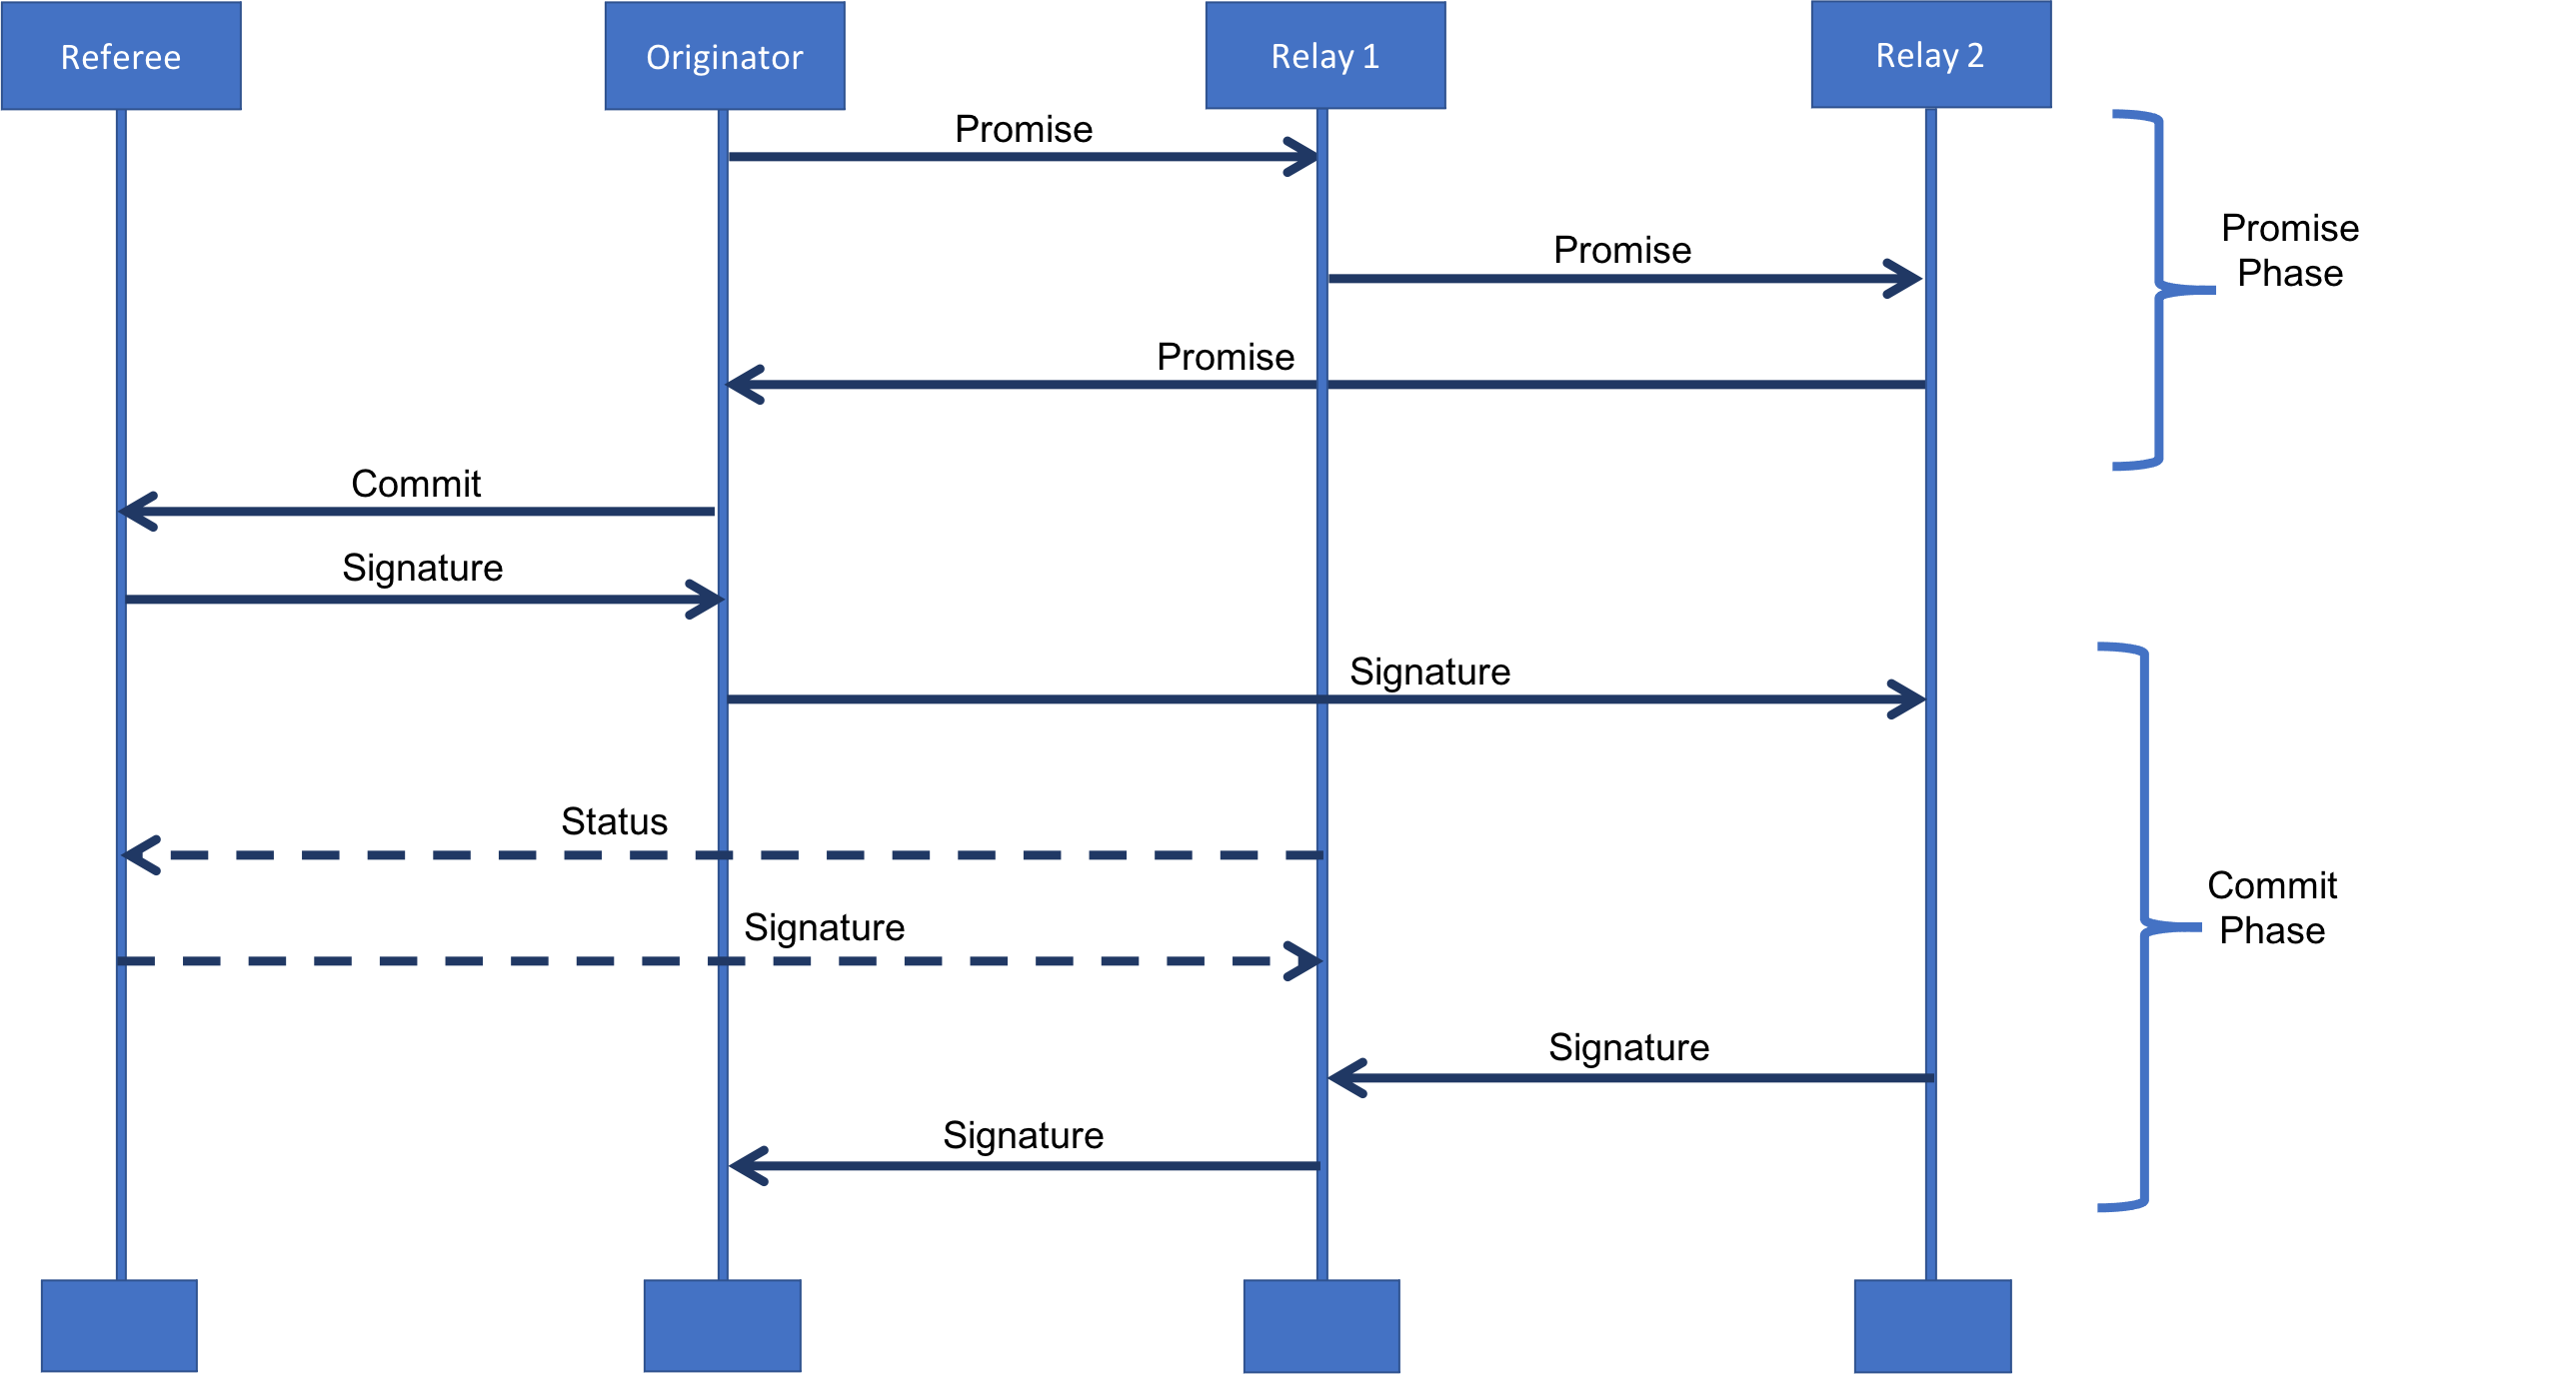
\includegraphics[scale=0.35]{SequenceDiagramLifeline.png}
    \caption{Lift Protocol Sequence Example}
    \label{fig:liftSequence}
\end{figure}

When Relay 1 receives the lift record, it first confirms that it trusts the referee to be fair and available, and it confirms that the timeout timestamp is acceptable. If the referee is not trusted, or the known route to the target is no longer valid (for instance if it was used in a different lift and the node no longer has debt on that route to clear) it may choose to not continue. The node can optionally return a message indicating that it does not intend to complete the lift, or the node can simply ignore the message and wait for the lift to timeout. In the model used for verification, nodes ignore messages if they do not intend to participate in a lift. In our example, Relay 1 wishes to participate, so it forwards the lift record along with its own promise to Relay 2. Relay 2 then similarly evaluates the lift and decides to forward a promise to its predecessor which happens to be the originator. 

When the originator receives the promise from Relay 2, the lift moves into the commit phase and the originator sends the lift record to the referee to request a signature to commit. 

When the referee receives a lift record with a request to commit, it checks its clock to see if it received the commit message before the timeout. If it received the commit message after the timeout, the Referee signs a statement nullifying the lift. If it received the commit message before the timeout, the referee signs the lift record and returns its signature to the originator. In either case, it records its result to provide to any node that requests the status of the lift. In the sequence diagram in Fig. \ref{fig:liftSequence}, the referee decides the commit message was received in time and sends the originator its signature.

When the originator receives the signature, it sends it to its successor in the circuit (Relay 2). Whenever a node in the circuit receives the signature, immediately the CHIPs it promised to its successor are valid. (i.e. it has forgiven the debt of its successor). 
To recover this value, it sends the signature to its predecessor.

In the sequence shown in Fig. \ref{fig:liftSequence}, once Relay 2 receives the signature, it experiences a long delay. Because of this delay, Relay 1 determines the lift is taking longer than expected and sends a message to the Referee to check the status of the lift. When the referee receives the status request, it checks its records and recalls the signature it previously provided to the originator. Because the lift is committed, the referee provides this signature to Relay 1. When a node receives a signature from the Referee instead of its predecessor it should not forward this signature. This ensures there is exactly one failure point in the cycle after which every node must obtain the lift status from the referee. This property is useful in proving the correctness of the protocol. However, eventually, Relay 1 receives the signature from Relay 2 which allows it to forward the signature. If the message sent by Relay 2 had arrived sooner, Relay 1 would not have needed to request the status from the Referee. Once the originator receives the signature from Relay 1, all nodes have received exactly the amount of CHIPs they have given and the lift is complete.

Note that the protocol makes a distinction between three roles nodes can take: originator, referee, or relay. In every lift, there is always exactly one originator, and exactly one referee, and there can be any number of relay nodes. These roles determine the types of actions a node can take and therefore define distinct equivalence classes to consider. 

\begin{figure}
    \centering
    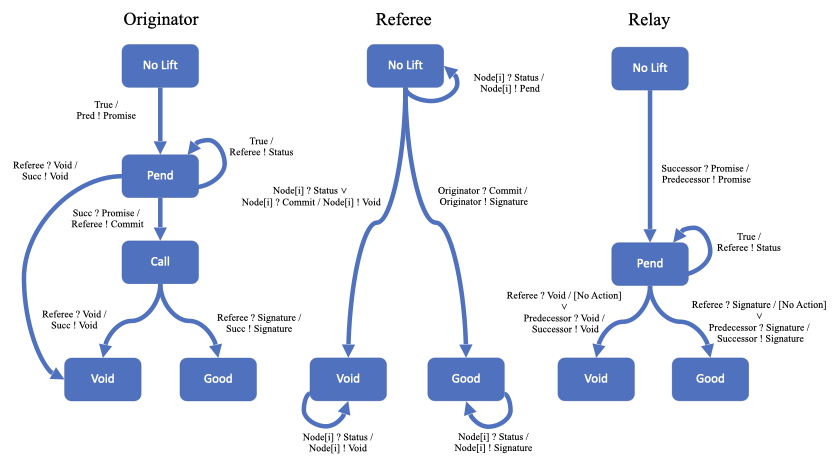
\includegraphics[scale=0.42]{LiftStatesSeperate.png}
    \caption{Lift States Diagram}
    \label{fig:liftStates}
\end{figure}

Fig. \ref{fig:liftStates} describes the behavior expected from each of these equivalence classes as mealy machines.
These mealy machines are based on the state machines Bateman provides to define the protocol \cite{bateman_state_machines}.
In the figure, each box represents the state of the lift from the perspective of the node, and each arrow represents a change in state and an associated action that is taken during the transition from one state to the next. Each transition is labeled with a condition that must be true for the transition to be taken, separated by a $/$ from an action that is taken during the transition. Each node has stored: the network ID of its predecessor (Pred), its successor (Succ), and the Referee. A transition can be made conditional on receiving a particular message from a particular network ID. This case is written in the form \emph{sender} $?$ \emph{message\_type}. As an action during a transition, nodes may transmit a particular message to a particular network ID. This case is written in the form \emph{recipient} $!$ \emph{message\_type}. 

The Spin model used as the model checking system is a direct implementation of the mealy machines in Fig. \ref{fig:liftStates}. The details of that implementation are described in Section \ref{chap:model_checking_results}. The set of rules for the proof in Coq are defined based on the mealy machine in Fig. \ref{fig:liftStates} and the sequence diagram in 
 Fig. \ref{fig:liftSequence}. Details of that implementation are described in Section \ref{chap:coq_results}.
 
\section{Extending model-checking results using an inductive proof}
\label{sec:extending}

We would like to prove that certain properties hold for a cycle of any number nodes using the MyCHIPs protocol.

\begin{theorem}[The properties hold on an arbitrarily large system]
The desired properties hold for an arbitrarily large number of nodes utilizing the MyCHIPs protocol.
$$
\forall n \in \mathds{N}, n \ge 1 \longrightarrow Prop(\emph{Ref}, \emph{Orig}, R_0, \dotsm, R_n)
$$
Where $Prop$ is a predicate that operates on a system of nodes operating under the MyCHIPs protocol. $Prop$ is applied to a system containing the required referee and originator singletons as well as a chain of 1 or more relay nodes.
\end{theorem}

To prove that these properties hold for an arbitrarily large system, we would like to construct an inductive proof. As the proof's base case, we will use a \emph{base system} that is small enough to prove our desired properties by an exhaustive search of the state space of the system. The proof's inductive step shows that the properties continue to hold when adding an additional node to a verified system.

\begin{lemma}[Base Case]
\label{lemma:base_system}
The properties hold for each node in a base system consisting of 1 referee, 1 originator, and 1 relay node.
$$
Prop(\emph{Ref}, \emph{Orig}, R_0)
$$
\end{lemma}

\begin{lemma}[Inductive Step]
\label{lemma:inductive_step}
$$
\forall n \in \mathds{N}, Prop(\emph{Ref}, \emph{Orig}, R_0, \dotsm, R_n) \longrightarrow Prop(\emph{Ref}, \emph{Orig}, R_0, \dotsm, R_n, R_{n+1})
$$
\end{lemma}

Lemma \ref{lemma:base_system} can be proven by an exhaustive search of the state space of the base system. This is accomplished using model checking as described in Section \ref{chap:model_checking_results}. Lemma \ref{lemma:inductive_step} can be proven---without the need to consider the individual properties---using conformance. Section \ref{sec:inductive_step} provides details of this method.

\section{Model Checking} \label{chap:model_checking_results}
We would like to prove that the properties hold on a base system consisting of 1 originator, 1 relay node, and 1 referee.
$$
Prop(\emph{Ref}, \emph{Orig}, R_0)
$$
The safety and liveness properties required for the MyCHIPs lift protocol can be proven by an exhaustive search all possible states in a small system. Spin is a powerful model-checking tool that allows for these types of properties to be expressed and verified. The state required by the system can be split into two classes: the part of the state that is evaluated when checking the properties, and the state that is used only to determine which state transition to take. We provide a formal definition of the former and a description of the latter. The source code for the complete spin model can be found on the \coderepository.
\subsection{Definition of the system state}\label{sec:statedef}
The system state is a combination of the individual states for each node. The state for the originator and each relay node can be represented as:
$$Node~state \equiv \langle S, B^s, B^p \rangle$$
$$
S \in \{\nolift, \pend, \call, \void, \good\}
$$
$$
B^s, B^p \in \mathds{Z}
$$
Here $S$ represents the mealy machine state and $B^s$ and $B^p$ represent the change in balance with the node's successor or predecessor respectively.

The state of the referee is similar except that it omits the balances
$$Referee~state \equiv \langle S \rangle$$

These are then composed together as a system state:
$$System~state \equiv \langle S_O, S_0, S_R, B^s_O, B^p_O, B^s_1, B^p_1 \rangle$$

With the $O$ subscript representing the \emph{originator}, $1$ representing the \emph{relay} node, and $R$ representing the \emph{referee}.

\subsubsection{Implementation of Node State Machines} 
Each mealy machine defined in Section \ref{sec:protocol_def} was implemented directly. This consisted of three process types: Originator, Relay, and Referee. Each process has a unique set of edges marked as non-deterministic choices that are enabled only when the current state $S$ matches the state of the edge in the diagram, and---if applicable---when the triggering message is present at the front of a message queue.


\subsubsection{Channels}
The message passing between nodes is modeled by creating 3 message channels for each node. One for messages received from the node's successor in the cycle, one for messages from the predecessor and one for messages from the referee. The referee also has a channel where it receives messages.

\subsubsection{Message Types}
The details of the message are not important for the model, instead, each message will have a specific type. It is expected that nodes in a real system will verify that messages are valid as part of processing a received message. For the model, we will consider invalid messages as if they were never received. Once a valid message is received, the type of that message will inform the actions a node will take in response to the message.

\subsubsection{Message Loss}
Rather than using the channels directly, the state machines for each node use helper functions to send messages. There are 3 functions: \emph{sendToPred} which sends a message to the predecessor in the cycle, \emph{sendToSucc} which sends to the successor, and \emph{sendToReferee} which sends to the referee. These helper functions determine which node the message should be sent to and puts the message in the appropriate channel. These helper functions also model the possibility that a message might be lost in transit.  One unique case is the possibility that all messages from a given node are dropped. This models the case where a node crashed or otherwise lost connection to the network. 

The protocol requires that the referee should be a node that is consistently available so messages to and from the referee are never dropped. This is required to prove some of the required liveness properties. Without this requirement, the problem is isomorphic with the \emph{two generals problem}, and it is impossible to guarantee eventual consensus on the lift status. This requirement enforces that eventually every message sent to and from the referee will be received, however, the model will evaluate the possibilities that arise should those messages take a very long time. 

\subsubsection{Modeling Time}
\label{sec:model_time}
Because we don't expect nodes to have synchronized clocks, modeling time for each node becomes extremely computationally complex. Rather than modeling time explicitly, we allow all decisions that would be made by a node based on time to be a non-deterministic choice. This allows the model to explore all combinations of clock-drift and all behavior that could arise without the need to model time. Leaving out time reduces the state space considerably and makes the analysis computationally feasible. 

\subsection{Definition of the properties}
The properties as described in in section \ref{sec:requiredProperties} are defined in terms of the simplified state presented in section \ref{sec:statedef}. 

\begin{definition}[Property 1]
\begin{multline*}
    P_1 \equiv \always\ \eventually,\\
    \originatorstate \neq \pend \wedge\ \relayastate \neq \pend \wedge\ \refstate \neq \nolift\\
\end{multline*}
\end{definition}
The purpose of $P_1$ is to verify that nodes are not left with a lift in an incomplete state forever. A node may be left unaware of a lift in the \nolift\ state or be in either the the \good\ or \void\ state. We make an exception that the referee must make a decision about any lift so the referee must not be left in the \nolift state. 

\begin{definition}[Property 2]
    
\begin{multline*}
P_2 \equiv \always\ \eventually, \\
    (\originatorstate = \good \leftrightarrow \relayastate = \good \leftrightarrow \refstate = \good) \\
\end{multline*}
\end{definition}
The purpose of $P_2$ is to verify that if any node belives the lift has completed and is in the \good\ state that all the nodes reach a consensus that the lift is \good. To show this we use a dual implication which ensures boolean equivilance. It is importatnt to note that the end states may be different if none of the nodes are in the \good\ state. For example, it is possible for $\originatorstate = \void\ \wedge\ \relayastate = \nolift\ \wedge\ \refstate = \void$.

\begin{definition}[Property 3]
\begin{multline*}
P_3 \equiv \always\ \eventually,\ \fair \longrightarrow \\
    (\originatorsuccbal + \originatorpredbal \ge 0) \wedge
    (\relayasuccbal + \relayapredbal \ge 0)\\
\end{multline*}
\end{definition}

The purpose of $P_3$ is to verify that the balance of every active node on the final state of the lift is equal to or greater than its initial balance. We record the change in a node's balance with its partners rather than its total balance. In a successful lift, we expect $B^s + B^p = 0$. However, if a node fails and stops transmitting, its successor might obtain the signature from the referee. When it does so it can use it to collect chips from its successor without needing to send chips to its predecessor. This is an allowable result so we allow $B^s + B^p \ge 1$.

\begin{definition}[Property 4]
\begin{multline*}
P_4 \equiv \always\ \eventually,\ \fair \longrightarrow \\
    (\originatorsuccbal = -\relayapredbal) \wedge
    (\relayasuccbal = -\originatorpredbal) \\
\end{multline*}
\end{definition}


The purpose of $P_4$ is to ensure that nodes are always in agreement with their partners on the change in the balance between them. 



\subsection{Results}

To verify each of these properties, Spin evaluated 
11478 unique states with 73805 edges between those states. Evaluating each property spin found that there were no counter-examples. 

From these results, we can conclude that the properties hold for a system with one originator, one relay node, and one referee, for all possible orderings and types of messages sent and for all combinations of messages failing to be delivered. This verifies Lemma \ref{lemma:base_system} as described in Section \ref{sec:extending}.

\section{Inductive Step}
\label{sec:inductive_step}

We would like to prove that the properties of a MyCHIPs system are preserved as it grows larger. 
$$
\forall n \in \mathds{N}, Prop(\emph{Ref}, \emph{Orig}, R_0, \dotsm, R_n) \longrightarrow Prop(\emph{Ref}, \emph{Orig}, R_0, \dotsm, R_n, R_{n+1})
$$
To prove this we would like to show that---in the context of a system of any size---a chain of 2 relay nodes $(R_n, R_{n+1})$ is a safe substitution for a single relay node $R_n$. By safe substitution, we mean that any behavior of $(R_n, R_{n+1})$ that could cause a failure is also a behavior of $R_n$. We can determine if this is true by observing the events (messages passed between nodes) in a given module and comparing them to the replacement module. These events and the order they occur are captured by a \emph{trace} of events. Dill explores the idea of \emph{traces} in the context of electrical circuits and developed \emph{trace theory} to reason about them. Dill's logic is often extended to reason about software and distributed systems. \krs{egm, is this true? I did a brief search and did not find many others using this... I can just remove this...} Dill describes a relation called Conformance that is used to determine when one module is a safe substitution for another \cite{dill_trace_theory}.
In Dill's work, he defines a sufficient condition for one module to conform to another:
$$F(R') \subseteq F(R) \wedge\ P(R) \subseteq P(R') \longrightarrow R' \preceq R$$
Where $F(R)$ is the set of traces that cause an internal failure in $R$, and $P(R)$ is the set of possible traces in $R$. 
The assumption is that if $R'$ experiences an internal failure the system as a whole will experience a failure. However, the goal of our analysis is to prove the properties of the system as a whole hold even when nodes in the system may fail. Because of this, there is no behavior of individual nodes that we will consider a failure. All of the behavior of each node, including the behavior of a node that experiences an internal error is considered in the possible behavior and not considered a failure. Written precisely:
$$
\forall R, F(R) = \varnothing
$$
This allows us to reduce the necessary condition for conformance to:

\begin{definition}[Conformance]
\label{def:conformance}
$$P(R) \subseteq P(R') \longrightarrow R \preceq R'$$
Where $P(R)$ and $P(R')$ are the sets of possible traces in $R$ and $R'$ respectively. 
\end{definition}

Dill's work allows us to admit the following theorem: 
\begin{theorem}[Conformance implies safe-substitution]
\label{theorem:dill}
 In the context of any system, if the component $R'$ conforms to the component $R$, then $R$ can be replaced by $R'$ and all properties of the system are preserved.
$$R' \preceq R \longrightarrow P(\dotsm, R, \dotsm) \longrightarrow P(\dotsm, R', \dotsm)
$$
\end{theorem}

Ideally, we would be able to directly prove that two relay nodes in a chain conform to a single relay node in the chain. In practice, this proof is complicated by the non-deterministic decision processes described in the mealy machines in section \ref{sec:protocol_def}. To simplify the proof we would like to hide the internal state of each node and instead focus on what is needed to prove conformance: the messages sent and received.

To do this we introduce an alternative implementation of the relay node $B$ that serves as a \emph{black-box} model. Rather than defining the node imperatively instead we describe the allowable inputs and outputs as a series of \emph{validity rules}. If properly defined, a black-box model $B$ will conform to the protocol definition $R$ and vice versa.

\begin{lemma}[Black-box conformance equivilance]
\label{lemma:ind_cof_model}
A relay node as defined by the \emph{validity rules} conforms to the node definition and the node definition conforms to the \emph{validity rules}.
$$B \preceq R\ 
\wedge\ 
R \preceq B$$
\end{lemma}

It is much easier to prove that a chain of two relay nodes conforms to a single relay node using the black-box model. 

\begin{lemma}[2 nodes conform to 1 node]
\label{lemma:chain_conform}
In the context of a MyCHIPs system, a chain of 2 relay nodes conforms to a single relay node for the black-box model.
$$\forall n \in \mathds{N}, (B_n, B_{n+1}) \preceq B_n
$$
\end{lemma}

In order for conformance to be provable, the alphabet of events that can occur in a trace from both modules needs to be equivalent. To enable this we define a standard interface that is sufficient for any number of relays in a chain. That interface includes 6 unique types of events:
\begin{enumerate}
    \item Promise Send
    \item Promise Receive
    \item Commit Send
    \item Commit Receive
    \item Status Send
    \item Status Receive
\end{enumerate}

The source and destinations for each of these messages are constrained by the protocol so these need not be included in the alphabet of events. Figure \ref{fig:blackboxsystem} illustrates these events.

Lemma \ref{lemma:ind_cof_model} considers two modules that each have exactly one relay node. Both modules take the form visualized in Figure \ref{fig:singlenodebox}. The first module contains a relay implemented using the mealy machine definition. The second module contains the model of the relay implemented using the \emph{validity rules}. Showing conformance equivalence between these two modules verifies that the two implementations match and can be interchanged freely without changing the behavior of the system. 

Lemma \ref{lemma:chain_conform} considers two modules where the first has exactly one relay node and the second has a chain of 2 (or more) relay nodes. These take the form of Figure \ref{fig:singlenodebox} and Figure \ref{fig:multinodebox}, respectively. In the second module, we introduce an \emph{Aggregator} which connects requests made from any node inside the module to a single external channel that communicates with the referee. We hide the details of the internal signals so that the alphabet of events matches the interface required for the black box. In a real system, the Referee will have some way of deciding which order messages are processed which fulfills this \emph{Aggregator} role. 
\begin{figure}
     \centering
     \begin{subfigure}[b]{\textwidth}
         \centering
         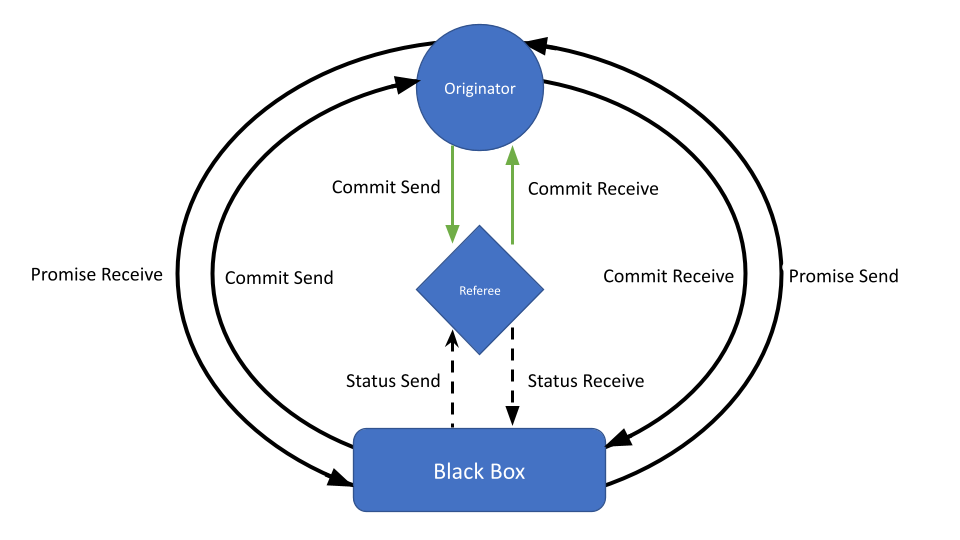
\includegraphics[width=\textwidth]{paper/SystemBlackBoxModel.png}
         \caption{Black Box System Model}
         \label{fig:blackboxsystem}
     \end{subfigure}
     \hfill
     \begin{subfigure}[b]{0.4\textwidth}
         \centering
         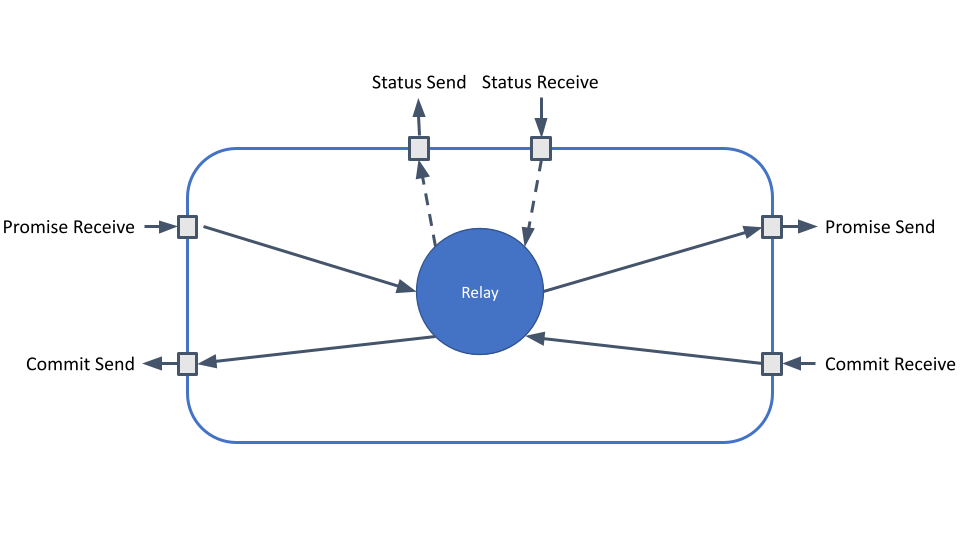
\includegraphics[width=1.4\textwidth]{paper/SingleNodeBlackBox.png}
         \caption{Single-node Contents}
         \label{fig:singlenodebox}
     \end{subfigure}
     \hfill
     \begin{subfigure}[b]{0.4\textwidth}
         \centering
         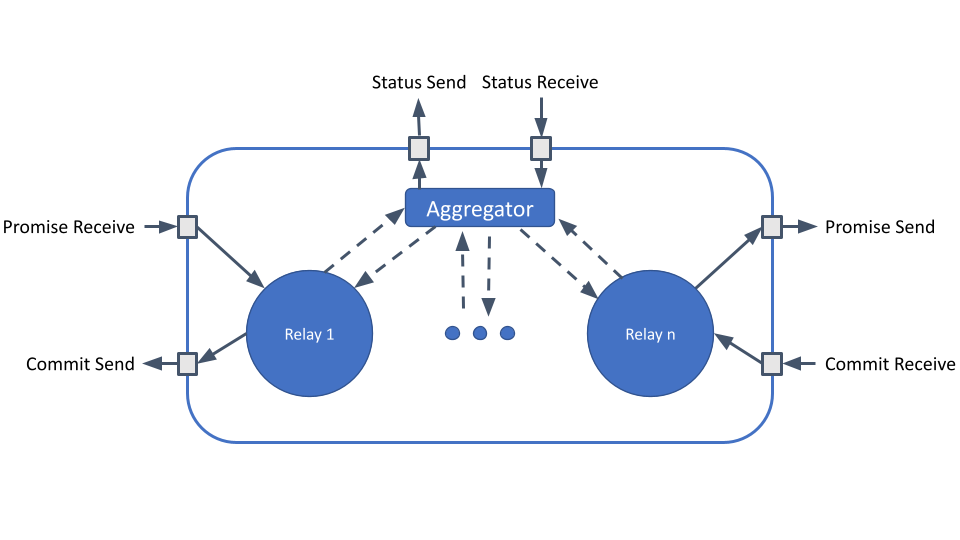
\includegraphics[width=1.4\textwidth]{paper/MultiNodeBlackBox.png}
         \caption{Multi-node Contents}
        \label{fig:multinodebox}
     \end{subfigure}
        \caption{Utilizing Conformance}
         \label{fig:allblackbox}
\end{figure}



Details of these implementations and proofs of conformance are presented in Sections \ref{sec:inputs_map} and \ref{chap:coq_results} to prove 
Lemmas \ref{lemma:ind_cof_model} and \ref{lemma:chain_conform} respectively.
Using Theorem \ref{theorem:dill}, and Lemmas \ref{lemma:ind_cof_model} and \ref{lemma:chain_conform} we can show:

\begin{manualtheorem}{\ref{lemma:inductive_step}}[Inductive Step]
Adding an additional node preserves the properties.
$$
\forall n \in \mathds{N}, P(\emph{Ref}, \emph{Orig}, R_0, \dotsm, R_n) \longrightarrow P(\emph{Ref}, \emph{Orig}, R_0, \dotsm, R_n, R_{n+1})
$$
\begin{proof}\ \\
    \vspace*{-20pt}
    \begin{multline*}
    P(\emph{Ref}, \emph{Orig}, R_0, \dotsm, R_n)\ \wedge\  B \preceq R\ \longrightarrow \\
    P(\emph{Ref}, \emph{Orig}, R_0, \dotsm, R_{n-1}, B_n)
    \end{multline*}
    \vspace*{-25pt}
    \begin{multline*}
    P(\emph{Ref}, \emph{Orig}, R_0, \dotsm, R_{n-1}, B_n)\ \wedge\  (B_n, B_{n+1}) \preceq (B_n)
 \longrightarrow 
    \\    
    P(\emph{Ref}, \emph{Orig}, R_0, \dotsm, R_{n-1}, B_n, B_{n+1})
    \end{multline*}
    \vspace*{-25pt}
    \begin{multline*}
    P(\emph{Ref}, \emph{Orig}, R_0, \dotsm, R_{n-1}, B_n, B_{n+1})\ \wedge\ R \preceq B\ \longrightarrow
    \\
    P(\emph{Ref}, \emph{Orig}, R_0, \dotsm, R_n, R_{n+1})
    \end{multline*}
    \vspace*{-25pt}
    \begin{multline*}
    \therefore  \forall n \in \mathds{N}, P(\emph{Ref}, \emph{Orig}, R_0, \dotsm, R_n) \longrightarrow P(\emph{Ref}, \emph{Orig}, R_0, \dotsm, R_n, R_{n+1})\ \qed
    \end{multline*}
\end{proof}
\end{manualtheorem}

\section{2 nodes conform to 1 node}
\label{chap:coq_results}

We would like to prove that a chain of 2 relay nodes conforms to a single relay node in the context of a MyCHIPs system as implemented in the inductive proof.
$$\forall n \in \mathds{N}, (B_n, B_{n+1}) \preceq (B_n)
$$

By Definition \ref{def:conformance} this is can be reduced to:
$$P(B_n, B_{n+1}) \subseteq P(B_n) \longrightarrow (B_n, B_{n+1}) \preceq B_n$$

The validity rules define the black-box model behavior by specifying all the possible traces of the model. A trace is a possible behavior of the model iff the trace meets all the validity rules:
\begin{equation}
\label{eq:valid_implies}
\forall T, \actsvalid{T}{n} \leftrightarrow
 T \in P(B_n)
\end{equation}

\begin{theorem}[Valid projection implies conformance]
\label{thm:valid_imp_conf}
$$
\left[ \forall T \in P(B_n, B_{n+1}), \actsvalid{\projectsize{T}{n}}{n} \right] \longrightarrow (B_n, B_{n+1}) \preceq B_n
$$
Where $\projectsize{T}{n}$ is a projection function that removes events from the trace that are not part of the alphabet of events in a system of size $n$. This is equivalent to a combination of \emph{hide} and \emph{renane} operations as described by Dill. 
\begin{proof}\ \\
Introduce: 
\begin{equation}
\label{eq:valid}
\forall T \in P(B_n, B_{n+1}), \actsvalid{\projectsize{T}{n}}{n}
\end{equation}
Assert:
\begin{equation}
P(B_n, B_{n+1}) \subseteq P(B_n)
\end{equation}
This is equivalent to:
\begin{equation}
\label{eq:subseteq}
P(B_n, B_{n+1}) \subseteq P(B_n) \equiv \forall T, T \in P(B_n, B_{n+1}) \longrightarrow T \in P(B_n)
\end{equation}
Apply (\ref{eq:valid_implies}) and (\ref{eq:valid}):
\begin{equation}
\forall T, T \in P(B_n, B_{n+1}) \longrightarrow T \in P(B_n)
\end{equation}
Apply (\ref{eq:subseteq}):
\begin{equation}
    \label{eq:goal2}
    P(B_n, B_{n+1}) \subseteq P(B_n)
\end{equation}
By Definition \ref{def:conformance}:
\begin{equation}
\therefore (B_n, B_{n+1}) \preceq B_n
\end{equation}
\qed
\end{proof}
\end{theorem}

\subsection{Machine-Checked Proof}
Coq is a popular interactive theorem prover that can be used to define and prove properties. Inductive reasoning techniques can be used in Coq to state and prove properties of arbitrarily large systems. 

We can use Coq to create a machine-checked proof that a chain of $n+1$ relay nodes can be projected onto a chain of $n$ nodes.
$$\forall T \in P(B_n, B_{n+1}), 
\actsvalid{T}{n+1} \longrightarrow
\actsvalid{\projectsize{T}{n}}{n}$$
The \emph{validity rules} and the \emph{projection} are formally defined in Sections \ref{sec:definitions} and \ref{sec:projection}. Section \ref{sec:proofs} describes the proof script.

The machine-checked proof script can be found in the \coderepository.

\subsection{Validity Rules Definition} \label{sec:definitions}
The MyCHIPs system in the Coq proof is written with a \emph{black-box} approach. The Coq proof does not need to know anything about the internal state of each of the nodes. Rather than considering each individual node in the system, the Coq proof operates on traces of all actions that might occur in the system. Each trace is represented by an ordered list of \emph{Actions}. The list represents the actions that each node took in the system in the order that they took them.

We define rules that must hold for a trace of actions to be considered valid. We define these rules such that all possible traces of actions in the system are considered valid, and all impossible traces are considered invalid. These rules include properties that are enforced by the MyCHIPs protocol as well as properties that are intrinsic to any distributed system. For example, we enforce  messages can only be received after the message has been sent.

\krs{We don't talk about ignoring PEND messages, but I think it just distracts from the message. We can probably omit it. Folks might ask because it is in the Mealy Machines}

Each node in the cycle has a unique ID represented by a non-negative integer. The Originator's ID is 0, with all other nodes in the system having some ID greater than 0. The referee does not have an ID but instead, the special SendRef and ReceiveRef actions are used for communication with the referee. 

\subsubsection{Validity Rules} \label{sec:validity_rules}
The rules that determine if a trace of actions is valid are defined in \emph{acts\_valid}. There are 8 rules:

\begin{enumerate}
  \itemsep 0pt
  \item \emph{has\_required\_actions}
  \item \emph{has\_no\_duplicate\_receives}
  \item \emph{all\_receives\_causal}
  \item \emph{all\_sends\_triggered}
  \item \emph{all\_ids\_in\_range}
  \item \emph{promise\_forward\_commit\_backward}
  \item \emph{phase\_sequence\_correct}
  \item \emph{all\_ref\_receives\_causal}
\end{enumerate}

All must hold for a trace of actions to be considered valid. The rules were designed to match the possible traces that could be generated by a system of nodes for the given size. All of these rules are defined formally below and described in detail in Appendix \ref{apdx:coq_detail}.

For the following definitions, we define an action type 
\begin{definition}[Action Type]
$$\action \equiv \{(Send, s, d, m), (Receive, d, m), (SendRef, s) (ReceiveRef, d)\}$$

Where $s \in \mathds{N}$ is the source identifier $0 \le s < size$, $d \in \mathds{Z}$ is the destination identifier $-1 \le d \le size$, and $m$ is a message $m \in \{\promise, \commit\}$.

\end{definition}
For the following definitions we use the notation: 
$T \equiv (a_1, a_2, ..., a_n), a_i \in \action,$ and denote the size of the system $S \in \mathds{N}$ which is a count of the number of nodes in the system.

\begin{definition}[has\_required\_actions] The trace contains the required Sends and Receives with Promise Messages, and nodes before a given failure point $m$ have the required Sends and Receives with Commit messages, or if they are after a given failure point they request the lift status from the referee.

$$
   \forall n \in \mathds{N}, n + 1 < S \longrightarrow \\
   (Send, n, n+1, Promise) \in T \wedge (Receive, n, Promise) \in T\ \\
$$
$$ \wedge \\ $$
$$
   \exists m \in \mathds{N}, \forall n \in \mathds{N}, \\
$$
$$
   (n \ge m) \longrightarrow (n + 1 < S) \longrightarrow \\
   (Send, n+1, n, Commit) \in T \wedge (Receive, n, Commit) \in T\ \\
$$
$$ \wedge \\ $$
$$
   (n < m) \longrightarrow (n < S) \longrightarrow \\
   (SendRef, n) \in T \wedge (ReceiveRef, n) \in T\ \\
$$
$$ \wedge \\ $$
$$
    (Send, 0, -1, Commit) \in T \\
$$
\end{definition}

\begin{definition}[has\_no\_duplicate\_receives]
The trace contains at most one of each receive action. 
$Given\ r = (Receive, d, m), n \in \mathds{N}, m \in \emph{Message},\ \sloppy{\sum_{T}[x=r]} \le 1$. Which counts the number of occurrences where $x=r$ in $T$. 
\end{definition}

\begin{definition}[all\_receives\_causal]
Every \emph{Receive} action is preceded by a corresponding \emph{Send} action. 
Given $r = (Receive, d, m), r \in T \longrightarrow \exists a = (Send, s, d^*, m), a \in T \wedge d^* = d \mod S \wedge a \happensbefore r.$ Where $\happensbefore$ is the happens-before relation over $T$, indicating that $a$ occurs before $r$ in the trace of events. 
\end{definition}

Because we allow the destination of a \emph{Send} to be an integer between $-1$ and the size \emph{inclusive} this means that a node can send a message with a destination $-1$ and this always corresponds with the node with the maximum ID in the system. Additionally, a node might send a message with the destination $n$, but when we project to size $n$ the node with ID $n$ is removed from the system. This send---instead of being sent to a node that doesn't exist---now gets mapped to node $0$ because the destination need only be equal modulo the size. This allows for the projection to work without the need to mutate actions, which makes proving properties about the projected system much simpler.  

\begin{definition}[all\_sends\_triggered] Only the originator sends a message without first receiving a message of the same type.
Given $a = (Send, s, d, m), a \in T \wedge s \neq 0 \longrightarrow \exists r, r = (Receive, s, m) \wedge r \in T \wedge r \happensbefore a$
\end{definition}

\begin{definition}[all\_ids\_in\_range] Ensures the trace only includes identifiers for nodes that are in a system of the given size. Destinations of a send are allowed to \emph{wrap} by one identifier. Given $a \in \action, a = (Send, s, d, m) \longrightarrow 0 \le s < S \wedge -1 \le d \le S$
\end{definition}

\begin{definition}[promise\_forward\_commit\_backward] All Promise messages are sent to the successor in the cycle and all Receive messages are sent to the predecessor. Given $a = (Send, s, d, m), a \in T \longrightarrow [(m = Promise \longrightarrow d = s + 1) \wedge (m = Commit \longrightarrow s = d + 1)]$
\end{definition}
\begin{definition}[phase\_sequence\_correct] The originator sends the first Commit message, and the originator is the last to receive each type of message. Given $a, b \in T$,
$$ 
a = (Send, 0, -1, Commit) \longrightarrow 
$$
$$
[
(b = (*, s, d, Commit) \wedge (s \neq 0 \vee d \neq -1) \longrightarrow a \happensbefore b)
\wedge 
(b = (Send, s, d, Promise) \longrightarrow b \happensbefore a)
]
$$
$$
a = (Receive, 0, m) \longrightarrow 
$$
$$
[
b = (Send, s, d, m) \longrightarrow b \happensbefore a
]
$$
$$
a = (SendRef, s) \longrightarrow 
$$
$$
[
b = (Send, s, d, Promise) \longrightarrow b \happensbefore a
]
\wedge
[
b = (Receive, s, Commit) \longrightarrow a \happensbefore b
]
$$
\end{definition}
\begin{definition}[all\_ref\_receives\_causal] No nodes receive a message from the referee before they have sent a message to the referee. Given $r = (ReceiveRef, d), r \in T \longrightarrow \exists a = (SendRef, d), a \in T \wedge a \happensbefore r$
\end{definition}


\subsection{Projection Definition}
\label{sec:projection}
Projection is defined with the \emph{projected} function. Given the size of the system we would like to project onto and an action, the \emph{projected} function determines if a given n action is kept or omitted in the projected trace. It uses a special type  
$option \action \equiv \{\emph{None}, \emph{Some a}\}$ with $a \in \action$.

\emph{projected} returns $\emph{None}$ if the given action, $a$,  should be omitted and $\emph{Some}\ a$ if the action should be kept in the projected trace.

\begin{definition}[projected]
\begin{multline*}
a = (Send, s, d, m) \longrightarrow \\
s \ge S \longrightarrow \emph{projected}(a, S) = \emph{None} \\
d > S \longrightarrow \emph{projected}(a, S) = \emph{None} \\
\end{multline*}
\begin{multline*}
a = (Receive, d, m) \longrightarrow \\
d \ge S \longrightarrow \emph{projected}(a, S) = \emph{None} \\
\end{multline*}
\begin{multline*}
a = (SendRef, s) \longrightarrow \\
s \ge S \longrightarrow \emph{projected}(a, S) = \emph{None} \\
\end{multline*}
\begin{multline*}
a = (ReceiveRef, d) \longrightarrow \\
d \ge S \longrightarrow \emph{projected}(a, S) = \emph{None} \\
\end{multline*}
\begin{multline*}
\emph{Otherwise} \longrightarrow \\
\emph{projected}(a, S) = \emph{Some}\ a\\
\end{multline*}
\end{definition}


\subsubsection{Mutations}
The type of the projected function would allow mutations of actions if necessary. Early attempts at the proof mutated actions to \emph{wrap} a sent message around to $0$ or $size-1$ when the destination was projected out. However, allowing actions to mutate as part of the projection increased the complexity of the proof. Using the modulo arithmetic construct to handle wrapping provides a more robust mathematical foundation. This allows for an implicit \emph{rename} during the projection. 

\begin{definition}[project\_to\_size]
Given a size and a list of actions, \emph{project\_to\_size}, denoted $\mathds{P}$, returns a new list of actions that omits all actions for which \emph{projected} returns None. 
$$
a \in T \wedge projected(a, s) = Some\ a \longrightarrow a \in \projectsize{T}{s}
$$
$$
projected(a, s) = None \longrightarrow a \notin \projectsize{T}{s}
$$
\end{definition}

\subsection{Proofs}
\label{sec:proofs}

The proof consists of a set lemmas that progressively build from basic principles to the main conformance property we would like to prove. This main theorem ensures that the set of messages sent and received for each node in the system is invariant with the size of the system. 

This main theorem is called \sloppy \emph{larger\_conforms\_to\_smaller} and utilizes many sublemmas to aid in the proof.
The \emph{stack} of supporting lemmas is visualized in Figure \ref{fig:coqLemmaStack}.
The symbols $\mathds{V}$ and $\mathds{P}$ are used for \emph{acts\_valid} and \emph{project\_to\_size} respectively. 

\begin{figure}[h]
    \centering
    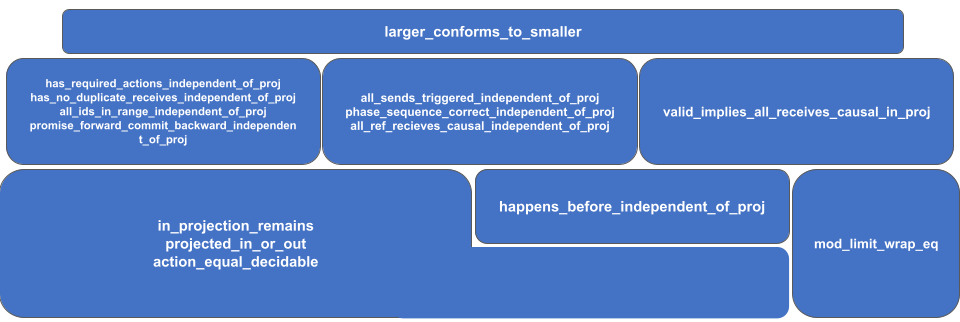
\includegraphics[scale=0.35]{CoqLemmaStack.png}
    \caption{Stack of Supporting Lemmas}
    \label{fig:coqLemmaStack}
\end{figure}

\begin{theorem}{larger\_conforms\_to\_smaller}
\label{thm:maintheorem}
$$\forall T \in \listaction\ \actsvalid{T}{n+1} \wedge n > 1 \longrightarrow \actsvalid{\projectsize{T}{n}}{n}.$$
\end{theorem}

The theorem \emph{larger\_conforms\_to\_smaller} is the main conformance theorem. It proves that all systems of size $n+1$ conform to a system of size $n$. This lemma relies on sublemmas that prove that most of the validity rules are independent of projection. Meaning if the rule holds in a system it continues to hold when projected to a smaller system. The only exception is the \emph{all\_receives\_causal} rule which is not independent of projection. Instead, we use a lemma \emph{valid\_implies\_all\_receives\_causal\_in\_proj} which shows that any valid system still maintains the \emph{all\_receives\_causal} rule in the projected system. Details of those proofs are described later in this section. 

%\begin{lemma}{project\_idempotent}
%$$\forall T \in \listaction\ n0\ n1 \in \mathds{N}, n0 < n1 \longrightarrow \projectsize{\projectsize{T}{n1}}{n0} = \projectsize{T}{n0}.$$
%\end{lemma}
%This lemma proves that projecting first to a larger size, $n$, then to a smaller size, $m$, is equivilant to projecting to size $m$ directly. This is proven directly through induction on the list of actions, and case analysis of each type of action. 
%The intuition is that actions are removed when one of their parameters is smaller then the size. Because $n>m$ we know that if an action was omitted in the projection to size $n$ then it also is omitted in the projection to size $m$.  

\begin{lemma}{has\_required\_actions\_independent\_of\_proj}
\begin{multline*}
\forall T \in \listaction\ n \in \mathds{N}, n > 1 \wedge \hra{T}{n+1} \longrightarrow \\
\hra{\projectsize{T}{n}}{n}
\end{multline*}
\end{lemma}


This lemma proves that if a trace of actions has all the required actions for size $n+1$ that implies that when that trace of actions is projected to size $n$ it also has all the required actions for size $n$. 

The intuition for this lemma is that the actions that are projected out are precisely the actions that are no longer required for the smaller system. The proof examines each type of action required by the smaller system and shows that the validity rules require that action in the larger system as well. This implies that the action exists in the original list. We then show that that action remains in the list after the projection.

\begin{lemma}{has\_no\_duplicate\_receives\_independent\_of\_proj}
\begin{multline*}
\forall T \in \listaction\ n \in \mathds{N}, n > 1 \wedge \hndr{T} \longrightarrow \\
\hndr{\projectsize{T}{n}}
\end{multline*}
\end{lemma}
This lemma proves that if a trace of actions does not have more then one receive to the same destination of a given type that implies that when the trace is projected to size $n$ it still has no duplicates.

This is proven by induction on the trace of actions, with the core intuition being that the projection can not introduce any new actions. This is proven in the sublemma \emph{not\_in\_orig\_not\_in\_proj}. 


\begin{lemma}{valid\_implies\_all\_receives\_causal\_in\_proj}
$$ \forall T \in \listaction\ n \in \mathds{N}, n > 1 \wedge \actsvalid{T}{n+1} \longrightarrow \allrc{\projectsize{T}{n}}{n} $$
\end{lemma}
This lemma is the least trivial and the core problem that needed to be proven to show that the larger system conforms to the smaller system. The receive causality property is difficult because a \emph{Send} action that is associated with a given \emph{Receive} in the original system may be removed in the projection. However, if the \emph{Send} for a \emph{Receive} is projected out there is an equivalent \emph{Send} from that node's predecessor that now can be matched with that \emph{Receive}. 

This lemma is proven by careful case analysis. The proof itself spans nearly 500 lines and makes use of information known about the trace of actions based on the \emph{acts\_valid} assumption. 

We begin by introducing an action $r$ which is the \receive\ in question. We assume it exists in the projected list and that it is indeed a \receive\ and use the sublemma \emph{in\_proj\_in\_orig} to show that the action must also appear in the original trace. 

With the knowledge that the action was in the original trace the assumption of the validity of the original trace allows us to show that there must be a corresponding \send\ for that \receive\ in the original trace. 

We now know that there is a \receive\ that is both in the original trace and in the projected trace and that there is a corresponding \send\ in the original trace. From here we examine the possible scenarios for what happens to the corresponding \send\ in the projection.

These scenarios are:
\begin{enumerate}
\item \label{case:normal} Both are unchanged. Neither the \send\ nor the \receive\ are removed and neither \emph{wrap} around in the modulus.
\item \label{case:src_wrap} The \send\ alone is projected out. The source of the \send\ refers to a node that is no longer in the system.
\item \label{case:dest_wrap} The \send\ destination alone is projected out and the send now \emph{wraps}.
\item \label{case:both_wrap} Both the \send\ source and the send destination refer to a node that is removed. 
\end{enumerate}


Scenario \ref{case:normal} is pretty straightforward, the \send\ for the \receive\ is the exact same \send\ as in the original trace. We just show that the send remains in the projection.

Scenario \ref{case:src_wrap} is tricky. The previously associated \send\ is now projected out. But the \receive\ is not projected out. To prove this scenario we use information about the required actions in the original trace. After unpacking this information we can show that there must be a \send\ that would have gone to the node that was projected out. We show that this \send\ \emph{wraps} due to the change in the size which means that that send is now associated with the \receive\ in question.

Scenario \ref{case:dest_wrap} is the dual of scenario \ref{case:src_wrap}. The same problem but from the other perspective. This is the case where a node that is not projected out sends to a node that is projected out. We show that that message \emph{wraps} to connect with a new \receive\ which is our \receive\ in question. 

Scenario \ref{case:both_wrap} is an interesting case because it is only possible if we project out more than one node in a single step. The way the property is defined this is not possible because we have a system that is valid for size $n+1$ that is projected to size $n$. It takes some mathematics and a few properties about modular arithmetic to show that this case is impossible and always leads to contradictions.

%Probably not worth mentioning here. They can see it in the script if they want.
%There is one final scenario in the proof not listed above. It is the case where the destenation of the receive is projected out. This comes out as an implementation detail for how we obtained some information about the original destination. We assumed that the original destination was either less then the new size or greater or equal to it. Then we checked each case. The case where the destination was greater or equal to the new size is easily dismissed by noting that that would mean that the recieve that needs a send was projected out, which is a contradicition with the assumption that it is in the projected trace.

Once each of these cases were individually proven or shown to lead to contradictions the property proves out.

\begin{lemma}{all\_sends\_triggered\_independent\_of\_proj}
$$ \forall T \in \listaction\ n \in \mathds{N}, n > 1 \wedge \allst{T} \longrightarrow \allst{\projectsize{T}{n}} $$
\end{lemma}
This lemma shows that if \emph{all\_sends\_triggered} holds in the original system it continues to hold in the projected system. This property enforces a partial order of events.

The intuition of this proof is that projections don't affect the order of events. This is proven concretely in the sublemma \emph{happens\_before\_independent\_of\_proj} which is used several times in this proof. 

\begin{lemma}{all\_ids\_in\_range\_independent\_of\_proj}
$$ \forall T \in \listaction\ n \in \mathds{N}, n > 1 \wedge \allir{T}{n+1} \longrightarrow \allir{\projectsize{T}{n}}{n} $$
\end{lemma}
This lemma proves that there are not any actions associated with nodes that would not be present in a system of the given size. It is directly poven based on the definition of \emph{projected}. 

\begin{lemma}{promise\_forward\_commit\_backward\_independent\_of\_proj}
\begin{multline*}
\forall T \in \listaction\ n \in \mathds{N}, n > 1 \wedge \pfcb{T} \longrightarrow \\
\pfcb{\projectsize{T}{n}} 
\end{multline*}
\end{lemma}
This property requires that the source and destination fields in Send actions follow certain patterns. The intuition of this proof is that projection does not mutate fields. We simply show that any projected item must have been in the original list. Because this property holds in the original list this property holds in the projected list.

\begin{lemma}{phase\_sequence\_correct\_independent\_of\_proj}
\begin{multline*}
\forall T \in \listaction\ n \in \mathds{N}, n > 1 \wedge \psc{T} \longrightarrow \\
\psc{\projectsize{T}{n}}
\end{multline*}
\end{lemma}
This property also imposes a partial order on traces. It is proven similar to \emph{all\_sends\_triggered\_independet\_of\_proj}, by showing that projections don't effect the order of events using the sublemma \emph{happens\_before\_independent\_of\_proj}. 

\begin{lemma}{all\_ref\_recieves\_causal\_independent\_of\_proj}
$$ \forall T \in \listaction\ n \in \mathds{N}, n > 1 \wedge \allrrc{T} \longrightarrow \allrrc{\projectsize{T}{n}} $$
\end{lemma}
This property requires that if a node receives a message from the referee it first sent a message to the referee. The intuition of this proof is that if a SendRef action that requested the status from the referee is projected out that implies that the ReceiveRef action is also projected out.

\begin{lemma}{not\_in\_orig\_not\_in\_proj}
$$ \forall T \in \listaction\ a \in \action\ n \in \mathds{N}, a \notin T  \longrightarrow a \notin \projectsize{T}{n} $$
\end{lemma}
This lemma shows that if an action is not in the original trace of actions it cannot be in the projected trace of actions. It is proven by induction on the trace of actions. It uses a proof by contradiction. We assume that the action is not in the original list but is in the projection. Then using the lemma \emph{in\_proj\_in\_orig}, we show that it must also be in the original list. This contradicts our first assumption.

\begin{lemma}{in\_proj\_in\_orig}
$$ \forall T \in \listaction\ a \in \action\ n \in \mathds{N}, a \in \projectsize{T}{n} \longrightarrow  a \in T $$
\end{lemma}
This lemma shows that if an action exists in the projected system then it must have existed in the original system. In other words, projection does not introduce new actions.
 It is proven by induction on the list of actions. The base case, an empty trace, easily leads to a contradiction. Then when considering a single action we use the definition of \emph{project\_to\_size} to show that the action must have come from the original trace. 

\begin{lemma}{happens\_before\_independent\_of\_proj}
$$ \forall T \in \listaction\ n \in \mathds{N},
a\ b \in T \wedge a\ b \in \projectsize{T}{n} \wedge a \happensbefore b \longrightarrow a \prec_{\projectsize{T}{n}} b
$$
\end{lemma}
This is the core lemma showing that projection doesn't reorder actions in the trace. It is proven by induction on the trace of actions. 

The base case, an empty trace, is easily dismissed with a proof by contradiction. 
Then when we consider a trace of actions with one additional action prepended to the trace. We call this new action $x$. On this new trace, we know that the action $a$ happens before the action $y$.
We can examine what might happen to $x$ in the projected trace.
We know that an action either remains in the projected trace or is removed entirely from the projected trace.
We will consider both of these cases.

If $x$ remains in the trace then it becomes the first item in the trace. 
We then consider the possible cases for what $x$ is.
$x$ could be equal to $a$, it could be equal to $b$, or it could be neither $a$ nor $b$.
If it is equal to $a$ then because it is the first item in the trace it must happen before $b$.
If it is equal to $b$ it means that $b$ must happen before $a$, however, $x$ is also the start of the unprojected trace so we can show that that is a contradiction with our assumption that $a$ happens before $b$ in the original trace.
If $x$ is neither $a$ nor $b$ then it does not have any bearing on whether $a$ happens before $b$ or not. We can then consider the rest of the trace to check that $a$ happens before $b$ in the subtrace. This reduces the problem to our inductive hypothesis.

Finally, we must consider the case where $x$ is removed from the trace in the projection. This immediately reduces to the inductive hypothesis which allows us to prove that the \emph{happens\_before} property is independent of projection.

\subsection{Results}
Theorem \ref{thm:maintheorem} tells us that the set of possible traces of actions taken by each node in a system is independent of the size of the system. Because this is true for a chain of n nodes we know that the possible traces of events in a chain of n nodes is equivalent to possible traces of events in a single node. With this and Theorem \ref{thm:valid_imp_conf} we know that a chain of n relay nodes conforms to a single node.
Thus we see that Lemma \ref{lemma:chain_conform} must be true:
$$\forall n \in \mathds{N}, (B_n, B_{n+1}) \preceq (B_n)
$$


\section{Conformance Equivalence of Black-Box Model}
\label{sec:inputs_map}
We would like to prove Lemma \ref{lemma:ind_cof_model}:
$$B \preceq R\ 
\wedge\ 
R \preceq B$$

By the Definition \ref{def:conformance} it is sufficient to prove:
$$P(B) \subseteq P(R) \wedge P(R) \subseteq P(B)$$

We will consider the left side and the right side of the conjunction separately. 
Sections \ref{sec:inputs_smaller} and \ref{sec:outputs_bigger} describe how the Spin model was adjusted to verify the left and right side respectively.

\subsection{The inductive proof's accepted inputs are a superset of the model-checking accepted inputs}
\label{sec:inputs_smaller}
If $P(B) \nsubseteq P(R)$ then there must exist a trace explored by Spin that breaks the validity rules. By encoding the validity rules as properties in Spin, we can then verify that the rules hold for all of the traces evaluated by Spin. 

To implement the properties the Spin model needed to be extended to generate a data structure that recorded the trace of actions. To simplify this structure we rely on the fact that messages received by nodes are \emph{idempotent}. If a node receives an message more then once the state will be the same as if it received the message only once. Because of this we can use boolean flags for each type of message at a given node, and make assertions about these booleans to verify the validity rules. The Spin model was adjusted to set these flags when a message was sent and when a message was received. 
After making these adjustments the validity rules can be written in Spin as properties, then Spin will evaluate each trace of events to ensure that the properties hold. 

When spin evaluates the system it considers all the possible ways that messages can be sent and lost. While all of these cases are captured by the validity rules, because the validity rules oprate on the trace of events in the system, if a node never sends or receives a message it is effectivly not in the system. This means that some of these cases are valid for size 0. Some of these cases are valid for size 1. And the rest of the cases are valid for size 2. Because we are primarily interested in verifing conformance between the black box model and the base system, we would like to write properties to verify the validity rules for size 2. 

However, when Spin verifies these properties it produces some counter-examples which correspond to a system of a smaller size. We would like to exclude these counter examples, so we introduce a new fairness property that eliminates cases that represent systems smaller than the base system. This property, \emph{size\_fair} requires that each node eventually leave the \emph{no\_lift} state. We then write each of the properties in the form:
$$size\_fair \longrightarrow property$$
After triggering on this fairness property, each of the validity rules verify for all traces evaluated by Spin. 

When adding a fairness property it is prudent to check that the fairness property can be met, otherwise we risk the properties verifying because they are vaccuously true. To ensure that the new \emph{size\_fair} property is achieved we write the property:
$$always\ !size\_fair$$
We expect this property to fail which indicates that the fairness constraint does not make our properties vaccously true. 

The implementation of these properties can be found in the \coderepository. After implementing the rules as properties Spin evaluated these properties and found no counter examples. These results verify that 
$P(R) \subseteq P(B)$. 

\subsection{The inductive proof's outputs are equivilant to the model-checking outputs}
\label{sec:outputs_bigger}
We would like to show:
$$P(B) \subseteq P(R)$$. 

We can examine all the possible combinations of messages for a single node to its predecessor, its successor, and the referee. Because a node might send more then one message of a given type this set is potentially infinitely large. We again rely on message idempotency in MyCHIPs. Because of this, the set of possible outputs we need to consider can be reduced into a small set of equivalence classes where each possible trace of events is represented by a canonical member that has only one of each type of message.

We can define these equivalence classes as an ordered list of actions with the property that each type of action appears in the list at most one time. 
We use the following abbreviations for the alphabet of events: 
\begin{enumerate}
    \item Promise Send $\equiv PS$
    \item Promise Receive $\equiv PR$
    \item Commit Send $\equiv CS$
    \item Commit Receive $\equiv CR$
    \item Status Send $\equiv SS$
    \item Status Receive $\equiv SR$
\end{enumerate}
For example: $[PR, SS, SR]$ is the case where the node receives a \promise\ but fails to send a promise then sends a \emph{status} request to the referee, then receives a status request.

Many of the possible orderings are not considered valid by the validity rules. For example, a node may only send a status after it has received a promise for the lift, a node must not request the status after it received a commit, and a node cannot send a commit until it has received a commit. 
After eliminating the impossible cases the remaining equivalence classes are:
\begin{enumerate}
    \item $[PR, SS, SR]$
    \item $[PR, PS, SS, SR]$
    \item $[PR, PS, CR]$
    \item $[PR, PS, CR, CS]$
    \item $[PR, PS, SS, CR, SR]$
    \item $[PR, PS, SS, SR, CR]$
    \item $[PR, PS, SS, SR, CR, CS]$
    \item $[PR, PS, SS, CR, SR, CS]$
    \item $[PR, PS, SS, CR, CS, SR]$
\end{enumerate}

We can evaluate if each of these equivalence classes is considered in the Spin model by generating a property that asserts a trace of that class is not present. If this property fails we know that the trace is evaluated at least once in the Spin model. If Spin verifies that each equivalence class is present then and we can conclude that Lemma \ref{lemma:ind_cof_model} holds.

Using the same adjusted model described in Section \ref{sec:inputs_smaller} we can write these properties as a never claim. Each never claim describes an automaton that accepts a trace of the respective equivalence class. When the automaton accepts the trace Spin produces an error indicating that the never claim was violated. We expect Spin to throw an error for each equivalence class and if it does we have verified that the equivalence class was explored in the Spin model. 

When executing the model checker with these never claims all of these equivalence classes are observed in the Spin model. This allows us to conclude that:
$$P(B) \subseteq P(R)$$

This together with $P(R) \subseteq P(B)$ as proven in Section \ref{sec:inputs_smaller} allows us to conclude:
$$B \preceq R\  \wedge\  R \preceq B$$
    
%\section{Assuring all nodes in the system are verified}
%\label{sec:nodes_map_base}
%We would like to prove Lemma \ref{lemma:all_nodes_covered}. 
%$$
%\forall N \in S, \exists N' \in \basesystem, \tracestruc{N'} = \tracestruc{N}.
%$$
%The core question asked by this Lemma is:
%Do all nodes in a large system have an analog in the base system?
%To prove this we need to show that we can construct a system with an arbitrarily large number of nodes by replacing nodes in the base system with a chain of n nodes such that an arbitrarily selected target node is a node that was originally in the base system.
%
%\egm{Move this into it's own section. Admit the lemma here, as needed for the proof, and in that later section, make the best argument possible and state that future work is to strengthen. The following paragraph and algorithm would go to that section.}
%\krs{Moved from Section 3 here}
%
%For example, if we would like to verify the properties hold for the node with ID 6 in a 15-node system, we construct a system where that node is unreplaced. To do this can choose to replace the originator with a chain of 6 nodes (including a new node with ID 0 to act as the originator). We then leave the first relay node in place as our desired 7th node (ID 6). Then we replace the second relay node with a chain of 8 nodes. We know that those substitutions are safe substitutions so we know the constructed system conforms to the base system. i.e. the target node cannot tell the difference between the base system and the newly constructed system. From this, we know that the properties hold for the target node. 
%
%This method can be generalized to construct a system of arbitrary size to verify the properties of an arbitrarily selected target. This generalization is described by Algorithm \ref{alg:const_ver}.
%
%
%\begin{algorithm}
%\caption{Constructing a verified system}
%\label{alg:const_ver}
%\begin{algorithmic}
%\State let $i \in \mathds{N}$ be the target ID, $s \in \mathds{N}$ be the target size.
%\If{$i = 0 \vee\ i=(s - 1)$}
%    \State Replace \emph{Relay 1} in base system with a chain of $(s - 2)$ nodes.
%    \State This is the verifying system.
%\Else
%    \State Replace the \emph{Originator} in base system with a chain of $i$ nodes.
%    \State Replace \emph{Relay 2} in the base system with a chain of $(s - i - 1)$ nodes. 
%    \State This is the verifying system.
%\EndIf
%\end{algorithmic}
%\end{algorithm}
%
%
%Because we can construct the system $S$ by replacing nodes in the base system without replacing an arbitrary target node, we can conclude:
%$$\forall N \in S, \exists N' \in \basesystem, \tracestruc{N'} = \tracestruc{N}$$.

\section{Related Work}
\krs{Need to add sections about other results that use conformance, as well as infinite state model checking}


There are numerous bodies of work that solve similar problems or utilize similar constructs. The following list is particularly relevant. 

\subsection{Infinate State Model Checking}
Clarke, Grümberg, and Browne describe a method for verifying properties on systems with many identical subprocesses. This method relies on a proof of bisimulation which is difficult to prove if these subprocesses can make non-deterministic choices as the nodes in the MyCHIPs system can. The method described in this work may have some isomorphism with their method but presents it in terms of conformance and other modern model-checking methods. 

German and Sistla build on the work of Clarke, Grümberg, and Browne, but present a fully automatic method that can reason about multiple identical processes without any manual proofs about those processes. 

German and Sistla's work is referenced by other papers describing methods for model-checking infinite state spaces. The methods at a high level make an adjustment to the state matching to weaken the equivalence relation. Two states may be unique due to some infinite variable (a natural number) being different but they are equivalent in all ways we care about for verifying a property. This allows the machinery that model checks state a system for liveness and safety properties to operate on an infinite state space. This is somewhat akin to abstract interpretation. 

\subsection{Digital Currency Background and Verification}
There are also several papers relating to digital currencies which may be helpful background when considering the MyCHIPs system described in Appendix \ref{apdx:mychips}.

 Nakamoto describes how transferable digital tokens can be double-spent. The paper introduces bitcoins and describes the proof of work method of overcoming this problem which is often referred to as blockchain technology. \cite{bitcoin} 

 Bateman recognizes that the double spending problem is present only in digital currencies that are both duplicatable and transferable. Blockchain technology prevents digital tokens from being duplicated. MyCHIPs instead is designed with non-transferable tokens. MyCHIPs utilizes credit lifts to allow these non-transferable tokens to be virtually fungible and to allow for effective transactions to be made. 
 
 Bhargavan et. al. Verify Smart Contracts \cite{SmartContracts}. Smart contracts are a type of distributed computation where the program that is executed is secured in a blockchain. While not directly related, smart contracts have the same financial stakes MyCHIPs have and some of their techniques could give inspiration.  Bhargavan et. al, translated the smart contract code into a functional programming language, F*, aimed at verification. This allowed for contract verification based on F* type-checking.

 \subsection{Proofs and methods for distributed systems}
 Fischer, Lynch, and Paterson,\cite{Fischer} prove the impossibility of consensus on even a Boolean, with even one faulty (or malicious) process. However, this is only true if the processes don't have synchronized clocks. This proof shows the necessity of the referee with strong reachability requirements for the lift algorithm to always eventually reach a consensus on if the lift should commit.
 
 Schneider summarizes and frames many fault-tolerant distributed algorithms in the framework of state machines\cite{StateMachine}. He shows how many common algorithms are isomorphic to, and can be derived using, the state machine approach. It is a helpful method to characterize and compare different approaches and this work is inspired by these methods.
 
 Lamport\cite{Lamport}, describes a refinement process that takes a distributed fault-tolerant consensus algorithm and hardens it to be tolerant of byzantine actors through a process he calls \emph{byzantizing.} This method may be useful in future work to ensure the MyCHIPs protocol follows key principles of Byzantine hard protocols.
 
 Delzanno, Tatarek, and Traverso, model check a common consensus algorithm called Paxos in Spin. Their spin constructs provide helpful examples of how distributed algorithms are efficiently modeled.\cite{Delzanno_2014}
 
 Konnov, Veith, and Widder explore the unsolved problems associated with model checking distributed algorithms. This can serve as a hazard map of difficult unsolved problems.\cite{Konnov}

\subsection{Work that uses similar methods for machine-checked proofs}
 Huang, Ogles, and Mercer prove that \emph{doesn't commute}, a weakened version of the happens-before relation, is sound for certain common classes of task parallel programs. They present a mechanized proof that proves properties for all traces constrained by a partial order. The methods demonstrated by Huang, Ogles, and Mercer were used as inspiration for some of this work's mechanized proofs. \cite{ben_DC}
 

\appendix

\section{The MyCHIPs system}
\label{apdx:mychips}
The MyCHIPs protocol and the methods used to verify it can be understood independently of the system it is used in. However, the curious reader will want to know more about the context in which the MyCHIPs protocol operates. This section provides an overview of the system. More details can be found on Kyle Bateman's website \cite{bateman_myCHIPs}. 
In particular, this section will cover the common challenges with using digital currency, how existing systems overcome those challenges, and how MyCHIPs overcomes those challenges in a unique way that provides additional benefits. 

\subsection{The two types of Money: Commodity and Credit}
The purpose of money is to be a medium of exchange, and it does so by storing value. When someone provides a good or service, the seller is usually given money in exchange. This money stores the value they provided until the seller is ready to redeem that value to get something they need.
For this to work, whatever is used as money needs to be considered valuable. There are two prevailing methods for accomplishing this: commodity money, and credit money. 

In this context, a commodity is anything that can be owned and that can have its right to ownership transferred from one party to another. A commodity derives its value from the economic laws of supply and demand. Because some commodities are consistently desired and are sufficiently scarce, their value is stable enough to be used as money. For example, gold has historically seen widespread use as commodity money. As long as a commodity is in demand and its supply is reasonably limited, it can likely be used as money.

In contrast, credit money exists as a promise from one party to another of future value--likely a commodity or service. If the party giving the promise is trustworthy, the credit money has value equal to what was promised.
%If not, such pledges may be secured by collateral, which is a promise of ownership of an existing commodity should the pledgor fail to deliver on the promise of future value. 

\subsection{Digital Currencies}
Most digital currencies, including Bitcoin and Ethereum \cite{bitcoin}, take the commodity money approach. This decision led to two key technical challenges: achieving scarcity, and community consensus on ownership.

\paragraph{Achieving Scarcity}
It can be difficult to make a digital object that can be kept scarce.
Physical commodities, such as gold, are difficult to locate and refine. To mirror this difficulty of discovery, a finite set of digital tokens can be mathematically defined in such a way that they were not known specifically in advance. However any token, once discovered, could be easily checked to determine if it belonged to the set. Furthermore, discovering tokens is often computationally complex enough that it requires significant time and energy to discover a new token. This allows for a commodity that is both digital and scarce.
There are many possible sets that could be used, however, hash functions and blockchains became the prevailing method because using this method simultaneously solves the community consensus problem.

\paragraph{Community Consensus}
For someone to transfer ownership of a commodity, it is important for them to be able to prove that they own the commodity. Because of this, using commodity-based money requires community consensus about who owns what commodities.

Community consensus can be difficult to achieve, especially when many malicious actors may be present. One frequently discussed example where community consensus is not successfully achieved is the \emph{double-spending} problem. \emph{Double spending} is a difficult challenge and efforts to solve the problem lead to the development of blockchain algorithms. 

\subsection{Double-Spending}
Double spending is a challenge that arises when using digital commodities as currency. To spend a commodity-based digital token, an entity must send a transmission that convinces a peer that it owns a digital token and is transferring ownership of that token to the peer. However, if the entity can send one transmission that fulfils this, it can easily send the same transmission to two peers simultaneously. If the peers have no means of communicating with each other (or some third party) then they each have no reason not to accept the digital currency. This allows a malicious actor to “double-spend” a digital token.

\subsection{Overcoming Double-Spending with a Public Ledger}
Most commodity-based digital currencies overcome the double-spending problem is using a public ledger. With a public ledger, each transaction between any entities using the digital currency must be stored in a single public record. By using a public record, double-spending can be identified and prevented. This public ledger may be implemented by assigning a central trusted authority to manage the ledger or it may use a decentralized ledger with a consensus algorithm. 

While using a central trusted authority to manage the ledger is simple, its centralized nature leads to certain risks. First, the central authority is a single point of failure. If the central authority experiences some error and is not able to process transactions for a period of time, all trade using the digital currency would halt. Second, giving the central authority control over all the transactions of a digital currency requires great trust in the authority. The central authority could easily falsify records in order to benefit itself or a third party. In practice, there is not a single authority that every potential user of a digital currency will consider worthy of that amount of trust.

Using a decentralized ledger removes the need for a single trusted authority, but steps must be taken to ensure that the ledger cannot be falsified by an attacker and that a quorum of users eventually agrees on the state of the public ledger. There are two common consensus algorithms used to achieve this: proof-of-work, and proof-of-stake.

\subsubsection{Proof-of-Work}
Proof-of-work consensus algorithms allow for a form of democratic consensus where the group that holds more then 50\% of the computational resources decides the state of the public ledger. The blockchain method accomplishes this by requiring each block to include a partial hash collision. Such a collision will includes a certain number of leading zeros in the result of the hash. Because cryptographic hash functions are designed to be unpredictable and non-reversible, there is no inverse function to compute what data must be added to a record to get the required hash. In order to add a block of data to the ledger an entity must compute many billions of hashes until it finds a partial collision. These blocks are then chained together so the hash of the previous block is included in the next block. 

By chaining these blocks together in order to make a change to a previous block that appears legitimate an attacker must recompute the hash collision for all subsequent blocks. If the attacker does not have more then 50\% of the computation power they won't be able to compute the required hashes faster then the block chain grows and will never be able to make a falsification appear legitimate.

This method has been quite successful at accomplishing its goals, but it has received criticism from the economic and environmental impacts it causes. In order to maintain security of the public ledger the computation work required needs to be great enough to prevent attacks, however computational work is not free. There is very large overhead to purchase and maintain equipment and supply power to be able to complete the computational puzzles required by proof-of-work. This means that transaction costs for block-chain currencies are much higher then traditional transactions. Additionally, the power used for proof-of-work often is generated by burning fossil fuels, which contributes to greenhouse gas emissions and depletes limited resources. Many argue that proof-of-work consensus algorithms are not sustainable. 

\subsubsection{Proof-of-Stake}
In response to these criticisms, algorithms have been implemented that rely on \emph{proof-of-stake} rather then proof of work. Proof-of-stake algorithms rely on similar principles as proof-of-work but rather then allowing anyone to complete the computational puzzle, validators are randomly selected from a pool. To become a validator an entity must place sufficient stake as collateral. If they are found to behave maliciously, their collateral is forfeit. This allows the computation puzzles to be set to be much easier to solve which in turn reduces the overhead and environmental impact of transactions.

\subsubsection{Public Ledgers and Privacy}
Both proof-of-work and proof-of-stake algorithms operate to create consensus on a single, public ledger. The requirement for a public ledger means that no transactions can be made privately. Steps can be taken to attempt to anonymouize transactions but if the identifiers used in the transaction are connected with the individuals they represent, anyone can see the entire history of that person's transactions. Additionally, requiring a consensus on a single public record limits how decentralized the digital currency can be. Because of the privacy concerns, the economic and environmental impact of blockchain transactions, and to make a more decentralized monetary system, an non-blockchain digital currency is desirable. MyCHIPs aims to serve as a credit-based digital currency that avoids these fundamental problems. 

\subsection{Private Credit Digital Currency}

Transferability is intrinsic to commodity money. If you cannot transfer ownership of the commodity you can't transfer the value and it doesn't work as money. Credit money however can be made non-transferable and still maintain value. The promise for goods or services connected with the credit money can be valuable even if that promise is valid only for you. Making tokens non-transferable solves many security problems but leads to other practical problems.

\subsection{Solving the double-spending problem with non-transferability}
To prevent double spending we must ensure that a malicious actor gains no benefit from transferring a digital token to two different peers. Rather then preventing duplication, MyCHIPs instead ensures that tokens are only transferred once. To meet this goal, tokens in the MyCHIPs system are designed to be non-fungible and non-transferable. A token is created for a single recipient and is valid for only that recipient. However, this method has an obvious problem: how does one spend a non-fungible, non-transferable token? MyCHIPs has a method to make CHIPs \emph{virtually fungible} that involves giving the CHIPs back to the issuer in a distributed algorithm called a credit lift.  \cite{bateman_myCHIPs}


\subsubsection{The value of a CHIP}
As mentioned above, blockchain based cryptocurrencies rely primarily on scarcity to drive their value.
Experience has shown how this results in highly volatile valuations over time.
Volatility may be useful in certain investments, but it is generally not desirable in a currency.

In the same way that bonds tend to be less volatile than stocks, a credit-based currency will be more stable than one based on a purely demand-driven commodity.
However, the credit lift algorithm does rely on the assumption that at each stage of the lift, parties are trading tokens that have a uniform nominal value.

This unit of measure is called the CHIP--a clever backronym for Credit Hour in Pool.
The value of a CHIP is defined to be the value of one hour of unskilled labor. Parties agree to this definition in a digital contract when they issue CHIPs. Recent research has placed this value at \$2.53. \cite{bateman_chip_value}

However, if a laborer is providing tools, or has some expertise in the work they may be able to negotiate receiving more than one CHIP for an hour worth of work.
That is up to the market to decide.
The CHIP definition only quantifies what is being promised with the issuance of each new CHIP.

Unfortunately, it is not very common where the seller of a good wants something directly from the buyer in exchange. To make MyCHIPs useful to facilitate trade the seller needs to be able to use the CHIPs to get goods or services from other entities besides the buyer. This is accomplished through a \emph{credit lift} (hereafter, \emph{lift}).

\subsection{Chits and Tallies}
Because a Token in the MyCHIPs is only valid between exactly two entities, these tokens only need to be tracked by those two entities. These tokens are tracked on a consensed record called a \emph{Tally}. A \emph{Chit} is an atomic transaction where one or more CHIPs are given to the partner. A Tally is an ordered collection of Chits with additional information to note the terms of the two entities agreement. 

Whenever a pair of entities desires to establish a trade relationship with each other, they create a new Tally to track that relationship. Most trade relationships are fairly consistent about who is selling goods or services and who is buying. When creating a Tally the entities establish this normal flow by assigning the entity who is usually paid and provides goods the \emph{Stock} role in the Tally, and the one who usually pays the \emph{Foil} role. These names hearken to a traditional method of tracking such credit relationships called a \emph{Split Tally}. If the entity that takes the \emph{Stock} role wishes to purchase goods or services from the \emph{Foil} entity, the entities create a new Tally with the roles reversed.

Each time a transaction is made, the entity with the Foil role creates a Chit that includes: 
\begin{enumerate}
    \item The number of CHIPs being sent
    \item A verifying digital signature
    \item The date and time of the transaction
    \item Other metadata about the transaction
\end{enumerate}
The verifying signature could be either the signature of the entity with the Foil role or as described in section \ref{sec:liftAlgorithm} the signature of the referee if the transaction is part of a credit lift. The verifying signature is all that is needed for one entity to prove the other owes some debt, however, it is helpful for both entities to have assurances that they are in agreement about the balance of their tally. 

To ensure that both entities agree on the state of the Tally, they exchange hashes of their Tally. If the hashes match they can be assured they are in agreement on both the Chits in the tally as well as the order of those Chits. If there is a mismatch, the consensus algorithm is simple: the Tally of the entity with the Foil role is considered correct. If there are still missing Chits, the entity with the Stock re-transmits those to the Foil. The Foil adds those Chits to the Tally and re-transmits its new hash. 

\subsubsection{The MyCHIPs Credit Lift}
A lift makes CHIPs \emph{virtually fungible} by identifying a circuit where every entity holds CHIPs issued by their predecessor in the circuit. The lift algorithm arranges for each entity in the cycle to forgive the debt of their predecessor to get the same amount forgiven by their successor. 
 
\begin{figure}[h]
    \centering
    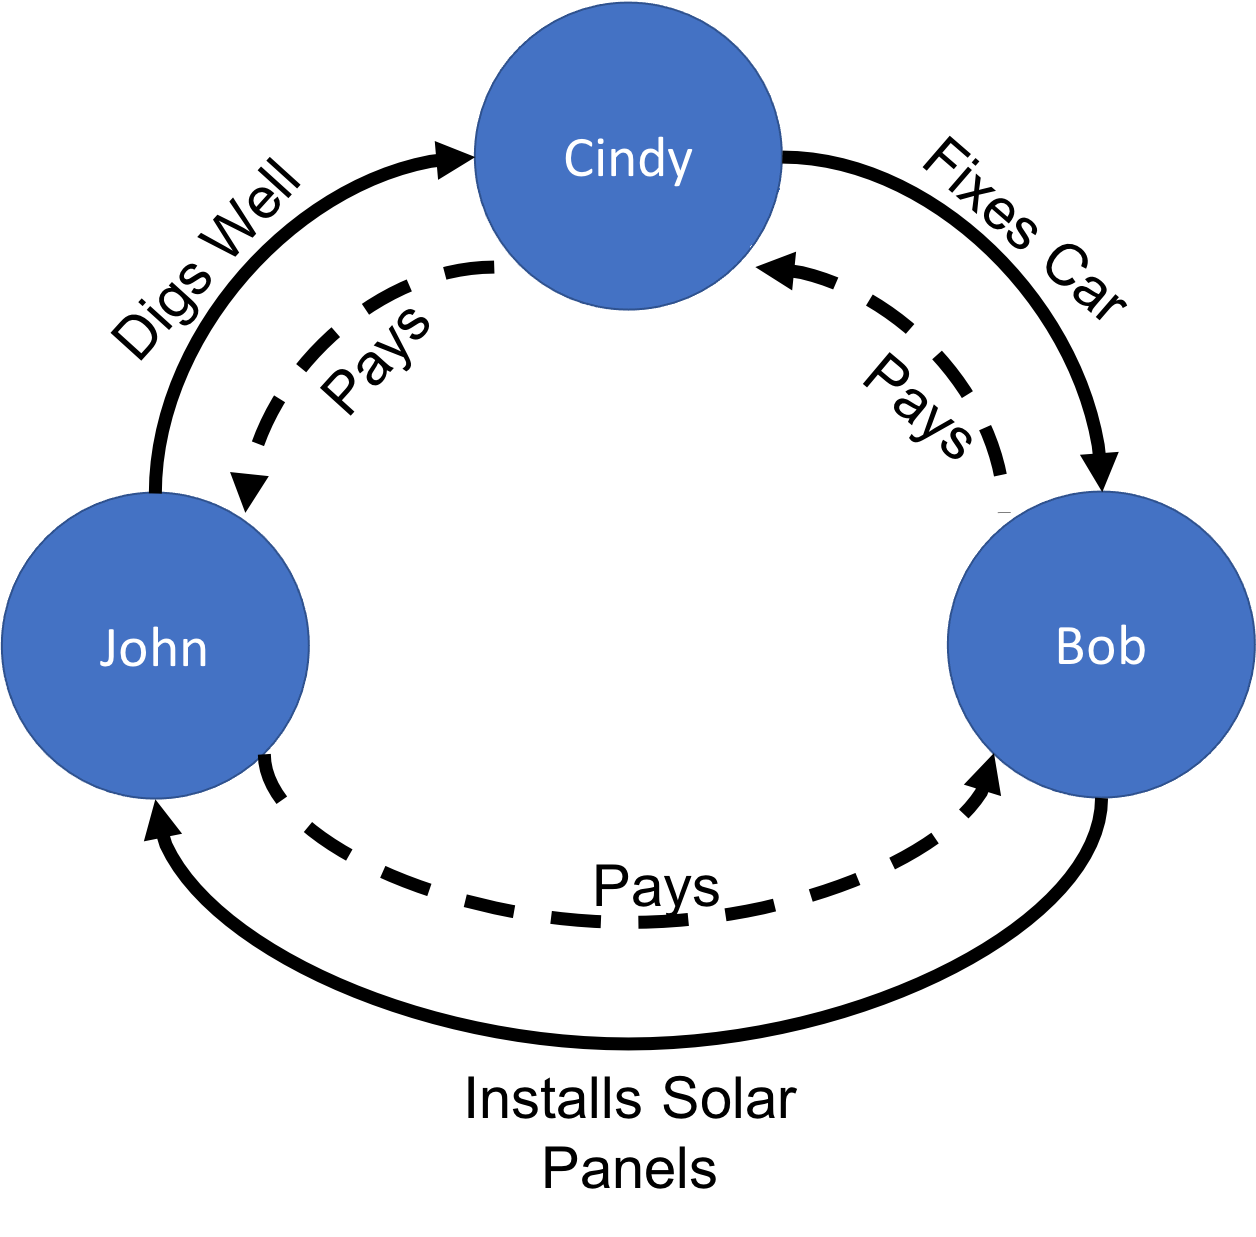
\includegraphics[scale=0.3]{ExampleCircuit.png}
    \caption{Example Circuit}
    \label{fig:liftProt}
\end{figure}
How this facilitates trade can be better understood by considering a barter system that involves more than two parties. 
For example, Bob needs his car fixed, John wants solar panels installed on his roof, and Cindy wants a well dug. Cindy knows how to fix cars, Bob knows how to install solar panels, and John is able to dig a well. See Fig. \ref{fig:liftProt} for a graphical representation of this arrangement. If they get together, they can work out a trade where John digs the well for Cindy, Cindy fixes Bob's Car, and Bob installs John's solar panels. Everyone would be happy.

But it is difficult to identify the these cycles before every transaction. This is where money comes in. Using government-backed money like dollars or euros, the process for enabling this transaction might go as follows:
\begin{enumerate}
\item Bob gets a loan from a bank
\item Bob uses the money from the loan to pay Cindy to fix his car.
\item Cindy gives that money to John to dig the well
\item John gives Bob the money to install the solar panels
\item Bob uses the money to repay his loan (but he may need to pay a little 
interest).
\end{enumerate}

MyCHIPs solves the same problem but instead does so by explicitly finding these cycles of value. Each person providing goods or services accepts CHIPs as an IOU for the exchange. Then a successful lift discovers this cycle of value and clears the debts of all involved.

If John, Bob, and Cindy were to use a credit lift to facilitate the arrangement it would go as follows:
\begin{enumerate}
\item Bob asks Cindy to fix his car and agrees to give Cindy 10 CHIPs 
\item Cindy gives John 10 CHIPs to dig the well
\item John gives Bob 10 CHIPs to install the solar panels
\item Cindy talks with Bob and learns that John gave Bob 10 CHIPs
\item Cindy realizes that Bob gave her 10 CHIPs, she gave John 10 CHIPS and John gave Bob 10 CHIPs. There is a cycle!
\item Cindy initiates a lift and \emph{promises} Bob that she will forgive his debt if he can get John to do the same for her. By doing this she takes on the role of the \emph{originator} of the lift. 
\item Bob gives John a similar promise.
\item John gives Cindy a similar promise and Cindy knows the deal is on.
\item Cindy \emph{commits} and gives Bob 10 CHIPs to cancel his debt
\item Bob gives John 10 CHIPs
\item John gives Cindy 10 CHIPs
\end{enumerate}
Everyone's tally for how many CHIPs they have given each other now totals to 0.
We can see this exchange allows for virtual fungibility: each person trades some CHIPs they have received to get back some CHIPs they have given out. 
This resets their balances so they can then give more CHIPs out again in exchange for future goods they will need. 

\section{Details of Coq Definitions}\label{apdx:coq_detail}

\paragraph{has\_required\_actions}
The has\_required\_actions rule is designed to check that the set of traces has all of the actions required by the protocol for a system of a given size. There are two sections to this rule that correspond with the promise and commit phase of the protocol. 

For the promise phase, we ensure that each node in the system receives and sends a promise message. In a real system, some messages may be lost which would cause some nodes to not receive a promise message, however, these cases can be considered to be a system of size $n$, where $n$ is the number of nodes who did receive a promise message. 

For the commit phase, we define a failure point $m$. Each node after $m$ may not receive a commit message and must send a status request to the referee. Each node before $m$ must receive a commit message. This failure point is an important construct for some of the required lemmas to prove the main theorem. To maintain this, a real system must not forward a signature obtained directly from the referee. 

The has\_required\_actions rule enforces a minimum requirement for actions that must be present in the trace, additional actions are permitted.

\paragraph{has\_no\_duplicate\_receives}
The has\_no\_duplicate\_receives rule is designed to check that is only one Receive action for each destination and message type. This rule simplifies the \emph{all\_receives\_causal} rule by allowing it to require only that there exists a corresponding send that happens before. Without this rule it would be necessary to match a corresponding send with each receive to ensure that one sent message is not received twice. This would make the proof much more complex. It is a property about how traces should be recorded. A real system must ensure that all responses to a message are idempotent or that duplicate received messages are ignored. 

\paragraph{all\_receives\_causal}
The all\_receives\_causal rule is designed to check that each receive is preceded by a corresponding send. To define this rule we define \sloppy \emph{is\_send\_for\_receive} which given two actions evaluates if the first is a Send and the second is a receive such that the destination of the send is equivalent to the destination of the receive. The equivalent here is defined as equal modulo the size of the system. This allows for messages that \emph{wrap} around the cycle to be considered equivalent without the need to mutate actions during projection. 

We also define a happens\_before function which evaluates to true only if the first action given occurs earlier in the list then the second action. 
Using these two definitions we can check to ensure that every Receive action is preceded by a corresponding send. 

\paragraph{all\_sends\_triggered}
The all\_sends\_triggered rule is designed to check that only the originator sends a message without first receiving a message that triggered that action. This rule again uses the \emph{happens\_before} function to check that that the triggering message is received before the triggered message is sent. 

\paragraph{all\_ids\_in\_range}
The all\_ids\_in\_range rule enforces the size of the system. It defines the allowable values for IDs in source and destination fields. All source fields must be a integer greater or equal to 0 and less then the size of the system. All destination fields can be up to one ID beyond the limit to allow for wrapping. This allows for destinations to be integers greater or equal to -1 and greater or equal to the size. However, messages received from the referee never wrap so they have the same rules as source fields. This property is necessary to identify and discriminate some invalid cases in some Lemmas. 

\paragraph{promise\_forward\_commit\_backward}
The promise\_forward\_commit\_backward rule enforces that promise messages are sent only to successors in the cycle, while commit messages are sent only to predecessors in the cycle. This rule also enforces that if a message wraps around the destination id must be greater then the size or less than 0 rather than using the equivalent id within range. This allows for wrapping messages to easily be identified and preserves monotonicity.

\paragraph{phase\_sequence\_correct}
The MyCHIPs lift protocol operates in two distinct phases, the promise phase, and the commit phase. The phase\_sequence\_correct rule enforces that the originator initiates these phases with the Promise phase first and the commit phase second. This property helps to discriminate invalid situations in some Lemmas.

\paragraph{all\_ref\_receives\_causal}
The all\_ref\_receives\_causal rule is similar to all\_receives\_causal but is is connected with messages to and from the referee. Because there is no need for destination ids to wrap this property is easier to define and prove. 

%%
%% The next two lines define the bibliography style to be used, and
%% the bibliography file.
\bibliographystyle{splncs04}
\bibliography{krs_thesis}


\end{document}
\endinput
%%
%% End of file `sample-acmtog.tex'.
